\section{Preliminaries}
\label{sec:Introduction}

\subsection{Introduction}

In the context of finite elements, construction of higher order shape functions for elements forming the exact sequence has been a long standing activity in both engineering and numerical analysis communities.
A comprehensive review of the subject can be found for example in \citet{hpbook}, \citet{hpbook2} and references therein.
%It suffices to say, that they are of fundamental importance in the implementation of all $p$ and $hp$ finite element methods.
%but cite only references relevant to the constructions presented in this report.

This document presents a self-contained systematic theory for the construction of a particular set of hierarchical, orientation embedded, $H^1$, $H(\mathrm{curl})$, $H(\mathrm{div})$, and $L^2$ conforming shape functions for elements of ``all shapes'', forming the 1D, 2D, and 3D commuting exact sequences discussed within.
By elements of ``all shapes'', we specifically mean the segment (unit interval) in 1D, the quadrilateral and triangle in 2D, and the hexahedron, tetrahedron, prism (wedge) and pyramid in 3D.

\begin{figure}[!ht]
\begin{center}
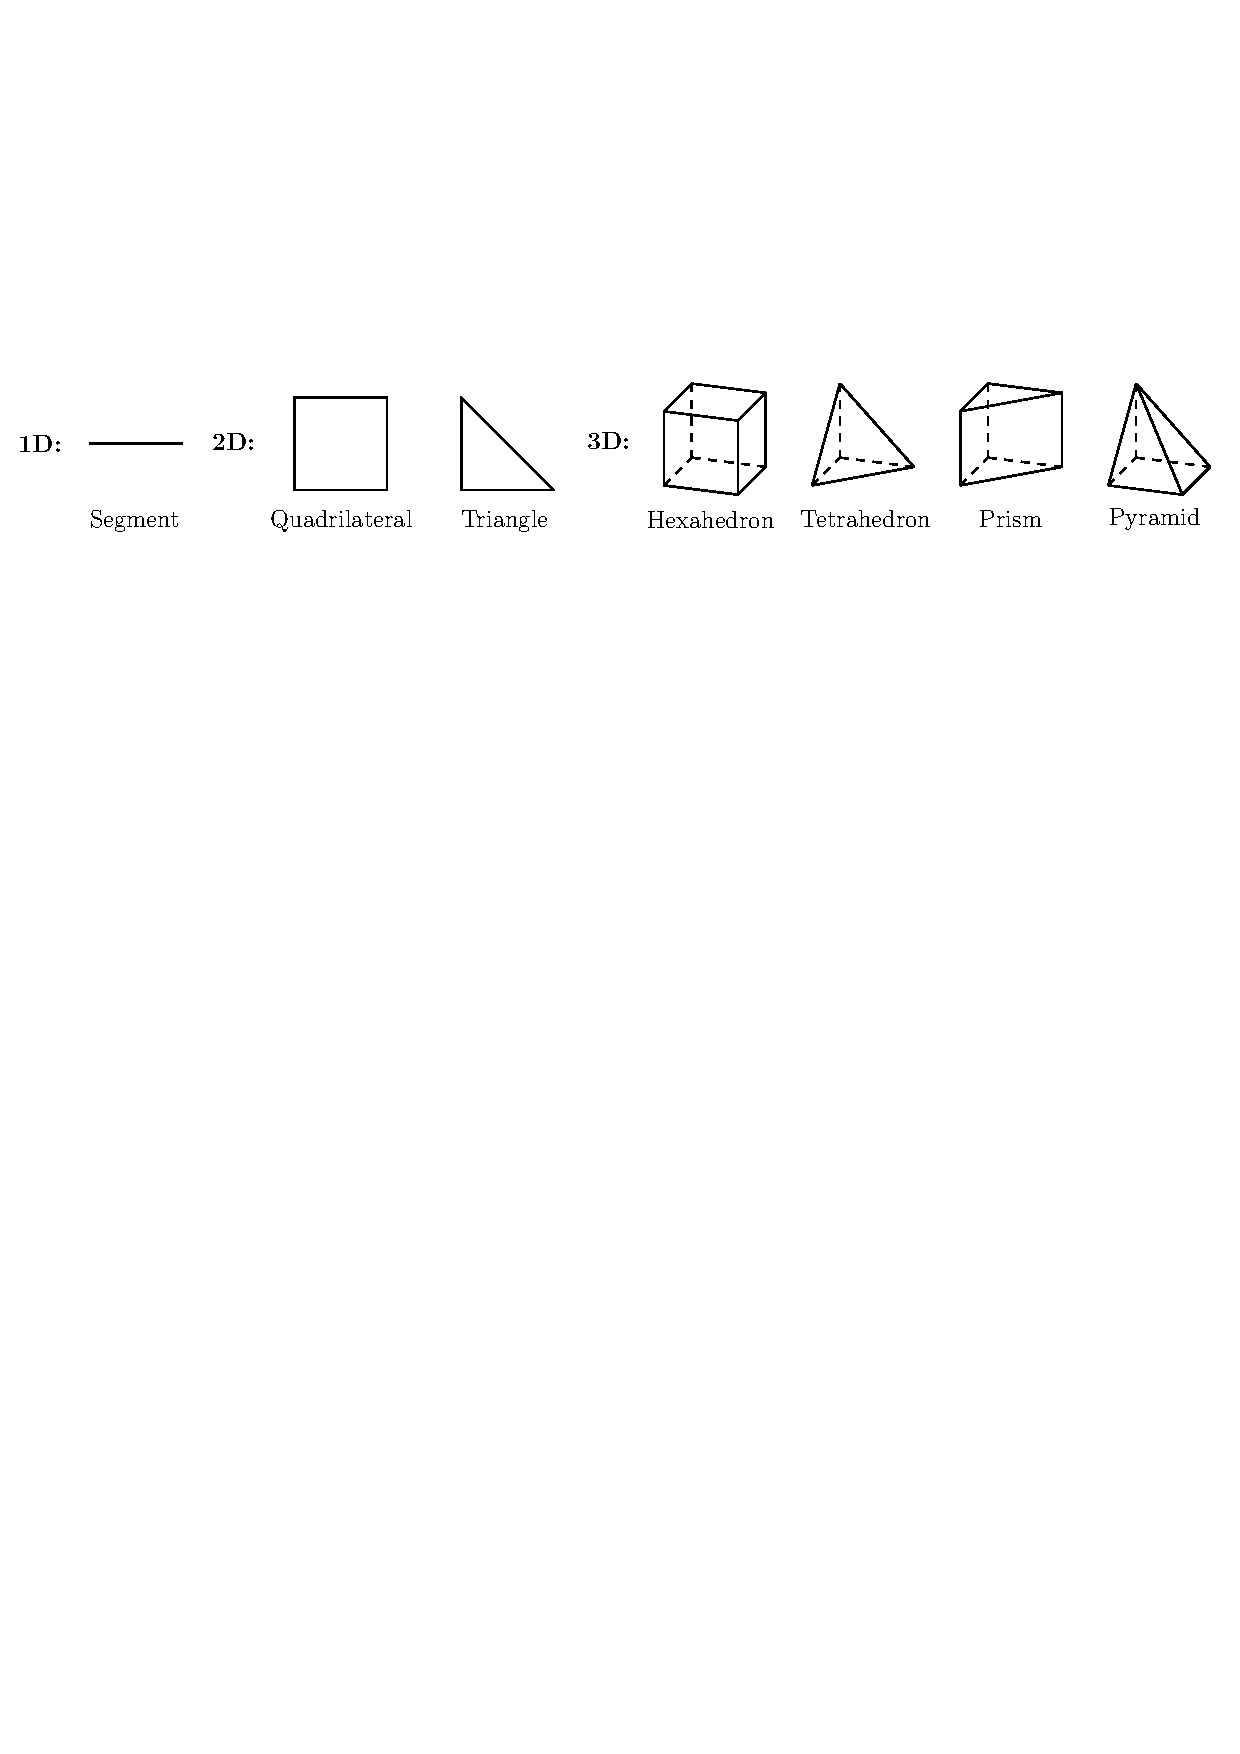
\includegraphics[scale=0.75]{./figures/ElementsAllShapes.pdf}
\caption{Elements of ``all shapes''.}\label{fig:elementsallshapes}
\end{center}
\end{figure}

There are many ways to construct sets of shape functions satisfying the aforementioned properties.
%We remind the reader that the performance of shape functions depends upon the particular problem being solved. % Therefore, there is no optimal or unique condition we may attribute to shape function construction in the generality preseneted in this paper.
However, we believe that in this work we have constructed a set which strikes an uncommon balance between simplicity and applicability. %\footnote{For instance, $H^1$ and $L^2$ shape functions for the triangle and tetrahedron which we derive are the same as those which appear in the work of \citet{Beuchler_Pillwein_Schoeberl_Zaglmayr_12} where they have shown good sparsity properties and also good conditioning for the stiffness and mass matrix.}
For all elements, and each associated energy space, we rely upon a simple methodology and a very small collection of ancillary functions to generate all of our shape functions.
Furthermore, we have supplemented this text with a package written in Fortran 90 defining each function presented in this work.\footnote{See the ESEAS library available at https://github.com/libESEAS/ESEAS.}
For these reasons, when reproducing our work in their own software, the readers should find the burden of implementation minimal.
We hope that our exposition will be clear and useful, particularly to those less familiar with the subject.

%This document presents a theory behind a stand alone package  that contains routines evaluating % Hereafter we will take freedom to use Finite Element (FE) jargon referring frequently to hexas and tets.

%The targeted audience for this document is less the colleagues contributing to the subject, who know it very well, but more a general computational science audience that may not be familiar with subtle mathematical details.
% We take thus some place not only to present specific constructions but also motivate them and place in a larger context. Throughout the document, we will not use boldface notations for 2D or 3D vectors (or vector-valued functions). These should be deduced from the context in which they are used.

For those at the forefront of shape function construction, we hope that our work will be intriguing if only for the elegance of our construction.
Particularly, we evidence \S\ref{sec:Pyramid} on pyramid shape functions.
The higher order discrete commuting exact sequence for this element appeared only recently in the work of \citet{Nigam_Phillips_11}.
Our construction for the pyramid presents shape functions spanning each of their discrete energy spaces while maintaining compatibility with the other 3D elements.
%With regards to $H(\mathrm{div})$, we believe this is the first construction presented in the literature which respects those pyramid higher order spaces.
We also remark that, for any given mesh, our shape functions are fully compatible across adjacent interelement boundaries due to considering so-called orientation embeddings.
Hence, no alterations of the shape functions are necessary at the finite element assembly procedure.
% orientation embedding (see \S\ref{sec:introorientations} for a more detailed discussion).
%With regard to attaining full compatibility of the shape functions across adjacent interelement boundaries via orientation embeddings, 
%we remark that our construction is able handle these coordinate transformations almost effortlessly by simply permuting the entries of a few relevant functions.
Moreover, these orientation embeddings are handled almost effortlessly by simply permuting the entries of a few relevant functions.
%We also evidence the ease at which orientation embeddings are handled in the shape function we present. 
% We believe that our presentation comprehensively illustrates the geometric similarities in each of the elements of ``all shapes.''

With regard to the choice of geometry (shape and size) of master elements, we followed \citet{hpbook}.
However, one of the key points is that our construction naturally applies to any other choice of master element geometries.
%However, we note that our methods are robust enough to easily generalize to other master element geometries.
%Despite basing our shape functions on the geometry (shape and size) of master elements followed by \citet{hpbook},
Other specific choices we made when enumerating element vertices, edges, and faces, can also be modified with little effort to the preferences of the reader.
%Of course, this also holds true for any other specific choices we made when enumerating element vertices, edges, and faces, which if desired, can be modified with little effort.
% and this particular choice of geometry is exploited in our construction.
%We also make specific choices when enumerating element vertices, edges, and faces, and also when selecting local edge and face orientations.
%If desired, these

For completeness, we have chosen to thoroughly verify the mathematical properties and to give a sound geometrical interpretation of our constructions rather than only give the necessary shape functions to the reader.
We concede that due to the depth of our presentation, and the expanse of our coverage, our offense lies only in the length of this document.
However, in a sense, an abridged version of this work is already present in a set of tables summarizing all the shape functions.
These can be conveniently consulted in Appendix~\ref{app:ShapeFunctionTable}. %to appear shortly for those requiring less details in the mathematics.

 %Our specific choices are summarized in Appendix \ref{app:Enumeration}.


%\subsection{Preliminaries}

\subsection{Energy Spaces and Exact Sequences}
\label{sec:Exactsequences}
Let $\Omega\subseteq\mathbb{R}^N$, with $N=1,2,3$ be a domain.
One arrives naturally at the \textit{energy spaces} $H^1(\Omega)$, $H(\text{curl},\Omega)$, $H(\text{div},\Omega)$ and $L^2(\Omega)$ in context of various variational formulations, see e.g. Chapter 1 in \citet{hpbook2}, \citet{DemkowiczGopalakrishnan13_2} and \citet{DemkowiczClosedRange}.
Along with operations of gradient, curl and divergence (understood in the sense of distributions), these spaces form the so-called \textit{complexes}, i.e. the composition of any two operators in the sequence reduces to the trivial operator.
The 1D complex, where $\Omega\subseteq\R$, provides the simplest example:
\begin{equation*}
	\mathbb{R} \stackrel{\text{id}}{\longrightarrow} H^1(\Omega) \stackrel{\nabla}{\longrightarrow} L^2(\Omega)
	\stackrel{0}{\longrightarrow} \{ 0 \}\,.
	\label{eq:1D_exact_sequence}
\end{equation*}
%where $\Omega = (0,1)$.
Here, the symbol $\mathbb{R}$ denotes constant functions, and $\{0\}$ is the trivial vector space consisting of the zero function only. By using the name of \textit{complex}, we communicate two simple facts: a) the derivative of a constant function is zero, and b) the composition of derivative (in fact, any linear operator) with the trivial (zero) operator is trivial as well. Equivalently, we can express the same facts by using null spaces and ranges of the involved operators:
\begin{equation*}
	\mathsf{R}(\text{id}) \subseteq \mathsf{N}(\nabla) \quad \text{and} \quad
	\mathsf{R}(\nabla) \subseteq \mathsf{N}(0) \, .
\end{equation*}
If instead of inclusions above, we have equalities, then we say that the complex (sequence) is \textit{exact}. This is indeed the case for the simply connected domain $\Omega = (0,1)$. 
By using the name \textit{exact sequence}, we communicate more information: a) the derivative of a function is zero \textit{if and only if} the function is a constant, and b) the function $\nabla : H^1(\Omega) \to L^2(\Omega)$ is a surjection (onto). From now on, we remove mention of the first and final terms of the exact sequence. The two spaces $\mathbb{R}$ and $\{0\}$, and the operators $\text{id}$ and $0$, are always assumed to buttress each of the sequences we later present. Moreover, whenever possible, we absorb the $\Omega$ assignment within the notation of each energy space. The domain $\Omega$ will always be assumed to be a simply connected domain in the relevant $\R^N$.
% It is customary to simplify the notation and drop the first and last spaces along with the identity and trivial operators, with their presence understood implicitly. We then have the 1D exact sequence:

\paragraph{1D Exact Sequence.} We now present the first exact sequence of simply connected domains in $\R$:
% \begin{description}
%   \item[1D sequence:]
\begin{equation}
H^1 \stackrel{\nabla}{\longrightarrow} L^2\, .
\end{equation}
% \end{description}

\paragraph{2D Exact Sequence.} The exact sequence for simply connected domains in $\R^2$ is of the form
\begin{equation}
H^1 \xrightarrow{\,\,\nabla\,\,} H(\mathrm{curl}) \xrightarrow{\nabla\times} L^2 \,,
\label{eq:2DExactSeq}
\end{equation}
where $\nabla\times$ and $\times$ are understood in two dimensions:
\begin{equation}
    \nabla\times E=\nabla\times\begin{pmatrix}E_1\\E_2\end{pmatrix}
        =\frac{\partial E_2}{\partial \xi_1}-\frac{\partial E_1}{\partial \xi_2}\,,\qquad\quad
    E\times F=\begin{pmatrix}E_1\\E_2\end{pmatrix}\times\begin{pmatrix}F_1\\F_2\end{pmatrix}
        =E_1 F_2 - E_2 F_1\,.\label{eq:2Dcurlandcross}
\end{equation}
By ``rotating'' $H(\mathrm{curl})$, the space $H(\mathrm{div})$ arises naturally:
\begin{equation}
    H(\mathrm{div})=\Big\{V_E=\Big(\begin{smallmatrix}0&1\\[2pt]-1&0\end{smallmatrix}\Big)E=
        \Big(\begin{smallmatrix}E_2\\-E_1\end{smallmatrix}\Big):
            E=\Big(\begin{smallmatrix}E_1\\E_2\end{smallmatrix}\Big)\in H(\mathrm{curl})\Big\}\,.
\label{eq:Hdiv2Ddef}
\end{equation}
Defined in this way, the ``rotated'' exact sequence is immediately satisfied:
\begin{equation}
H^1 \xrightarrow{\mathrm{curl}} H(\mathrm{div}) \xrightarrow{\,\nabla\cdot\,} L^2 \,,
\label{eq:2DExactSeqRotated}
\end{equation}
where, for all $\phi\in H^1$ and all $E\in H(\mathrm{curl})$, the operations satisfy the following relations: %$\mathrm{curl}\,(\phi)$ is understood as
\begin{equation}
    \mathrm{curl}\,(\phi)=\begin{pmatrix}\frac{\partial\phi}{\partial \xi_2}\\[4pt]-\frac{\partial\phi}{\partial \xi_1}\end{pmatrix}
        =\begin{pmatrix}0&1\\[4pt]-1&0\end{pmatrix}\nabla\phi\,,\qquad\quad
            \nabla\cdot V_E=\nabla\cdot\begin{pmatrix}0&1\\[4pt]-1&0\end{pmatrix}E=\nabla\times E\,.
\end{equation}


% For a simply connected domain, $\Omega \subset \mathbb{R}^2$, we have two exact 2D sequences:
% % \begin{description}
%   % \item[2D sequence:]
% \be
% H^1(\Omega) \stackrel{\bfnab}{\longrightarrow}
% H(\text{curl},\Omega) \stackrel{\text{curl}}{\longrightarrow}
% L^2(\Omega) \, ,%\quad \text{and,}
% \label{eq:2D_exact_sequence}
% \ee
%   % \item[Rotated 2D sequence:]
% and its rotated analogue,
% \be
% H^1(\Omega) \stackrel{\bfnab \times }{\longrightarrow}
% H(\text{div},\Omega) \stackrel{\bfnab \cdot}{\longrightarrow}
% L^2(\Omega) \, .
% \label{eq:2D_rotated_exact_sequence}
% \ee
% % \end{description}
% The operators curl and $\bfnab \times$ seen above are defined as follows:
% \be
% \text{curl} (E_1(x_1,x_2),E_2(x_1,x_2)) = \frac{\ptl E_2}{\ptl x_1} - \frac{\ptl E_1}{\ptl x_2}
% \quad \text{and} \quad
% \bfnab \times u(x_1,x_2) = \left(
% \frac{\ptl u}{\ptl x_2}, - \frac{\ptl u}{\ptl x_1} \right) \ .
% \label{eq:2D_curl_operators}
% \ee
% It is easy to see that the rotated sequence is obtained from the original one by rotating the coordinates,
% $(x_1,x_2)\mapsto(x_2,-x_1)$. The main point of the rotated sequence is that there is no need for a separate
% construction of 2D $H(\text{div})$ shape functions that can be obtained from 2D $H(\text{curl})$ shape functions
% by using the formula:
% \be
% (V_1,V_2) = (E_2, - E_1) \, .
% \ee
\paragraph{3D Exact Sequence.} Finally, for a simply connected domain in $\mathbb{R}^3$, we have the 3D exact sequence
\begin{equation}
H^1 \xrightarrow{\,\,\nabla\,\,} H(\mathrm{curl}) \xrightarrow{\nabla\times} H(\mathrm{div}) \xrightarrow{\,\nabla\cdot\,} L^2 \, .
\label{eq:3D_exact_sequence}
\end{equation}
%Note that the 2D exact sequences are ``embedded'' in the 3D sequence if one considers the appropriate restriction to functions of only two variables.

For all elements, these exact sequences will be reproduced on the discrete level by replacing the energy spaces with appropriate polynomial subspaces.\footnote{Or rational polynomial subspaces in the case of the pyramid (see \S\ref{sec:Pyramid}).} We shall use the standard notation:
\begin{equation}
\begin{aligned}
	\text{1D}:&\quad\qquad W^p \xrightarrow{\,\,\nabla\,\,\,}Y^p \, ,\\
	\text{2D}:&\qquad\!\!\Bigg\{\begin{array}{c}
		W^p \xrightarrow{\,\,\nabla\,\,\,} Q^p \xrightarrow{\nabla\times} Y^p  \, ,\\[4pt]
		W^p \xrightarrow{\mathrm{curl}} V^p \xrightarrow{\,\nabla\cdot\,} Y^p  \, ,\end{array}\\
	\text{3D}:&\quad\qquad W^p \xrightarrow{\,\,\nabla\,\,\,} Q^p \xrightarrow{\nabla\times} V^p \xrightarrow{\,\nabla\cdot\,} Y^p\,.
\end{aligned}
\label{eq:polynomial_exact_sequences}
\end{equation}
The symbol $p$ loosely denotes the polynomial order and should not be interpreted literally.\footnote{By this we mean that $p$ should, in fact, be interpreted as a multi-index for the Cartesian product elements.}

In this work, we shall consider only spaces of the \textit{first type} which, with the exception of the pyramid, were introduced by \citet{Nedelec80} in the \textit{first} of his two famous papers.
The pyramid spaces were taken as the first set of spaces proposed by \citet{Nigam_Phillips_11}.
All these spaces satisfy a number of fundamental properties.
First, the spaces of the different elements are said be tracewise \textit{compatible} at the level of spaces.
This allows them to be used in \textit{hybrid meshes}, which may contain elements of all shapes.
Second, for each element, $W^p$ contains polynomials of total order $p$, while $Q^p$, $V^p$ and $Y^p$ contain polynomials of total order $p-1$, meaning that the overall drop in polynomial degree from the first discrete energy space in the exact sequence to the last discrete energy space is one.
%That is, if the space $W^p$ contains polynomials of order $p$, then $Y^p$ contains polynomials of order $p-1$.
Thirdly, for a given element and energy space, the discrete spaces form a nested sequence of spaces as the order increases (for instance, $W^p\subseteq W^{p+1}$ and so on).
This is a necessary condition for the construction of hierarchical sets of shape functions.
Lastly, the spaces form \textit{commuting} exact sequences for each element.
This, coupled with the previous properties, ensures (global) interpolation estimates for \textit{all} of our energy spaces subject to affine transformations of the master element geometries \citep{monk_demkowicz}.

%With an outlook toward {\em hybrid meshes} that may contain elements of all shapes in one mesh, we require the spaces of the different elements to be tracewise \textit{compatible} at the level of spaces.
%Moreover, another desired property is that they form \textit{commuting} exact sequences for each element.
%This then ensures (global) interpolation estimates for \textit{all} of our energy spaces subject to affine transformations \citep{monk_demkowicz}.
%Finally, the discrete energy spaces (for a given element) should form a nested sequence of spaces as the order increases (for instance, $W^p\subseteq W^{p+1}$ and so on).
%This is a necessary condition for the construction of hierarchical sets of shape functions.
%In this work, all these properties are satisfied.
%We shall consider only spaces of the {\em first type} which, with the exception of the pyramid, were introduced by \citet{Nedelec80} in the {\em first} of his two famous papers.
%They present an overall drop in polynomial degree by one from the first discrete energy space in the exact sequence to the last discrete energy space.
%That is, if the space $W^p$ contains polynomials of order $p$, then $Y^p$ contains polynomials of order $p-1$.

%With these properties in mind, in this work  
%%The use of these spaces, is motivated with an outlook toward {\em hybrid meshes} that may contain elements of all shapes in one mesh.
%%To have such a mesh, the spaces of the different elements have to ``understand'' each other across the element boundaries.
%%If this is the case, they are said to be tracewise \textit{compatible} at the level of spaces.
%A common property of all these spaces is an overall drop in polynomial degree by one from the first discrete energy space in the exact sequence to the last discrete energy space.
%That is, if the space $W^p$ contains polynomials of order $p$, then $Y_p$ contains polynomials of order $p-1$.
%Moreover, another shared fundamental property is that they form \textit{commuting} exact sequences.
%This then ensures (global) interpolation estimates for \textit{all} of our energy spaces subject to affine transformations \citep{monk_demkowicz}.
%Finally, it is noted that the discrete energy spaces (for a given element) form a nested sequence of spaces as the order increases (for instance, $W^p\subseteq W^{p+1}$ and so on).
%This is a necessary condition for the construction of hierarchical sets of shape functions.

%the $H(\text{curl})$ and $H(\text{div})$ conforming N\'{e}d\'{e}lec and Raviart-Thomas spaces present in the exact sequences of the triangle and tetrahedral elements have the nice property that they are affine invariant.

%The second aspect of the exact sequence philosophy is a careful choice of discrete energy spaces. In our discrete exact sequences for the triangle and tetrahedral elements, we use the well known $H(\text{curl})$-conforming \Nedelec~and $H(\text{div})$-conforming Raviart-Thomas spaces.\footnote{See definitions for these spaces in \S~\ref{sec:Tri} and \S~\ref{sec:Tet}.} Unlike other higher order discete energy spaces used in the literature, these spaces happen to be affine invariant while also preserving a commuting exact sequence structure. In fact, we make the distinction that all of our discrete exact sequences preserve a commuting exact sequence stucture which  \textit{cite}

%In the $p$ or $hp$ FE methods, the order of approximation may vary from element to element and it may be different for each relevant topological entity (edge, face or element interior).
%That is reflected in the constructions presented in this report.
%The edge order must not exceed the order of adjacent spaces and the face order must not exceed the order of adjacent elements (see \citet{hpbook} and \citet{hpbook2} for discussions on the {\em minimum rule}).

%Unlike in \citet{hpbook,hpbook2}, we do not account in our notation for discrete spaces for variable order.

\subsection{Shape Functions}
We shall always identify the discrete spaces first (like $W^p$, $Q^p$, $V^p$ and $Y^p$ in \eqref{eq:polynomial_exact_sequences}), and only afterward introduce the corresponding shape functions that provide bases for those spaces.
This is a good place to remind the reader that there are, in fact, two competing schools of thought when it comes to the theory of shape functions.

%The classical definition of \citet{Ciarlet} starts with \textit{degrees of freedom} that are functionals defined on some large energy space $\mathcal{X}$ (like $H^1$).
The classical definition of \citet{Ciarlet} starts with \textit{degrees of freedom} that are functionals defined on some large subset $\mathcal{X}$ of an energy space $U$ (like $C^\infty\cap H^1\subseteq H^1$). 
The shape functions, which are elements spanning some discrete (finite dimensional) space $X\subseteq\mathcal{X}$ (e.g. $W^p\subseteq C^\infty\cap H^1$), are then defined as the dual basis to the linearly independent (when restricted to $X$) degrees of freedom.
An \textit{interpolation operator} from $\mathcal{X}$ to $X$ is then naturally defined.
In this construction, we must (usually) precompute the shape functions, e.g. in terms of combinations of monomials whose corresponding coefficients are stored.

%The classical definition of \citet{Ciarlet} starts with {\em degrees of freedom} that are functionals defined on some energy space $\mathcal{X}$ containing both the discrete trial space $X\subseteq\mathcal{X}$ and the exact solution. The degrees of freedom should be linearly independent when restricted to the finite dimensional domain $X$. The shape functions, which are elements of $X$, are then precisely the dual basis to the restricted degrees of freedom. An \textit{interpolation operator} is then intuitively defined. In this construction, we must (usually) precompute the shape functions in terms of combinations of monomials and then store the corresponding coefficients.

The competing approach of Szab\'o \citep{SzaboBabuska91} starts with a direct construction of shape functions by following a topological classification (of vertices, edges, faces and element interiors) induced by conformity requirements.
The shape functions are defined in terms of families of polynomials (e.g. Legendre) and their integrals, and are computed using simple recursive formulas. This is the approach taken in this work.
The so-called \textit{projection-based interpolation} \citep{hpbook,hpbook2} defined through local projections over element edges, faces and interior, is introduced \textit{independently} of the construction of shape functions.
Therefore, with no need to precompute coefficients defining the shape functions, following Szab\'o's approach is perhaps more convenient and straightforward.

\subsection{Hierarchy in \texorpdfstring{$p$}{p}}

Given an energy space (like $H^1$) and a conforming discrete space of order $p$ (like $W^p\subseteq H^1$), denote the shape functions forming a basis for the discrete space by $\mathcal{B}^p$ (e.g. $\mathrm{span}(\mathcal{B}^p)=W^p\subseteq H^1$). 
A construction is said to be hierarchical in $p$ if $\mathcal{B}^p\subseteq\mathcal{B}^{p+1}$ for all $p$, so that the set of shape functions spanning a space of a certain order is found in all subsequent enriched spaces of higher order.
This implies that as $p$ increases, all one has to do is to add a few functions to a smaller previously constructed set of shape functions.

%In our construction, hierarchy in the order $p$ of shape functions will be enforced.
%That is, the set of shape functions existing in a discrete energy space of a particular order (say $p$) will be found in all subsequent enriched discrete energy spaces of higher order, say $q\geq p$.
%For example, when constructing shape functions spanning $W^{p+1}$, all one needs to do is add a few functions to the smaller previously constructed set of shape functions which span $W^p$.
%%For example, let $p\geq1$ and let $W^p$ be the higher order discrete energy space conforming to $H^1$.
%%We will construct a set of shape functions spanning $W^{p}$ by simply adding to the smaller, previously constructed set of shape functions which span $W^{p-1}$.

In our construction, hierarchy in $p$ will be enforced. 
In a given mesh, it will allow comparison of shape functions between adjacent elements that have different order, so that at least some of the shape functions of the neighboring elements will match.
%More so, one can even have different orders for each topological entity (vertex, edge, etc.) independently.
This is crucial with regard to the notion of local $p$ adaptivity, which some methods employ.
In our work, this flexibility in the variability of the order will be partly reflected by the natural anisotropies present in Cartesian product elements, such as quadrilaterals, hexahedra and prisms, where each independent direction can have a different order.
More information can be consulted in the literature (see \citet{hpbook2} and references therein).


\subsection{Traces and Compatibility}
\label{sec:compatibility}
%Global conformity depends upon the energy space. More precisely, the requirements on the global continuity For instance, $H^1$-conforming shape functions must be globally continuous while the vector-valued $H(\text{curl})$-conforming shape functions must only be continuous in their tangential components across interelement boundaries. Similarly, for vector-valued $H(\text{div})$-conforming shape functions, only the continuity of only the normal component is enforced. In the final case, $L^2$-conformity does not involve any continuity assumptions at all.

%The global solution of any finite element method should satisfy certain conformity (continuity) properties, which clearly depend upon the energy space.
For a function to be contained in a given energy space it must satisfy some global conformity conditions which depend upon the space.
For instance, functions in $H^1$ are almost globally continuous, but functions in $L^2$ can be much more discontinuous.
%In the case of the vector valued $H(\mathrm{curl})$ and $H(\mathrm{div})$ spaces, there is a middle ground.

Due to these conformity requirements, each energy space has a different definition of \textit{trace} at the boundaries. 
%To be conforming to the energy space, functions should then be continuous at the trace level.
The different traces only make sense on certain parts of the boundary.
%and functions are said to be continuous at the trace level.
%This trace affects only certain parts of the boundary.
For instance, consider a polyhedral element.
%Polyhedral elementsthis means the functions should be (tracewise) continuous across interelement boundaries.
\begin{itemize}
	\item The $H^1$ trace is the value of the function itself at the boundary. In 3D, it may take values at element vertices, edges and faces which lie along the boundary.
	\item The $H(\text{curl})$ (tangential) trace is the tangential component of the vector valued function across the boundary. It may take values at edges and faces in the boundary, but not at vertices, since these do not have a concept of tangent. In fact, the $H(\text{curl})$ (tangential) trace is scalar valued across edges (which have 1D tangent spaces) and has two components across faces (which have 2D tangent spaces).
	\item The $H(\text{div})$ (normal) trace is the normal component of the vector valued function across the boundary. In 3D, it can take values at the faces of the boundary, but not at vertices or edges, since they do not have a unique notion of normal. In 2D, edges along the boundary \textit{do} have a notion of normal, so the (normal) edge trace does exist.
	\item There is no notion of trace for $L^2$.
\end{itemize}

%Different energy spaces also lead to different notion of {\em traces}. By the $H^1$ trace of a scalar-valued (sufficiently) regular function, we understand simply its restriction to the boundary. By the (tangential) $H(\text{curl})$ trace of a vector-valued function, we understand the restriction of its {\em tangential component} on the boundary. Thus, the  $H(\text{curl})$ trace of a two component function $(E_1,E_2)$ in $\mathbb{R}^2$ to an element edge, is going to be a scalar-valued function. In 3D, however, the trace of a 3D vector-valued function to an element face, will be a 2D vector. Similarly, the (normal) $H(\text{div})$ trace of a vector-valued function to an edge (2D) or a face (3D) is always a vector orthogonal to the element boundary that involves just one scalar component.

%Functions should then to be continuous at the trace level to .
At the discrete level, these considerations lead naturally to a classification of shape functions according to topological entities, which in turn depend on the number of spatial dimensions:
\begin{equation*}
	\begin{aligned}
		\text{1D:}&\quad\qquad\text{vertex and edge shape functions,}\\
		\text{2D:}&\quad\qquad\text{vertex, edge, and face shape functions,}\\
		\text{3D:}&\quad\qquad\text{vertex, edge, face and interior shape functions.}
	\end{aligned}
\end{equation*}

For any given mesh and energy space, shape functions of adjacent elements \textit{must} be continuous at the trace level across the shared interelement boundaries.
This is referred to as \textit{compatibility}, and results in the global conformity of the (disjoint union of) shape functions. 
For instance, in 2D, the order $p$ edge shape function of a quadrilateral would need to be compatible with the order $p$ edge shape function of an adjacent triangle (see Figure \ref{fig:compatibilitydefinition}).

\begin{figure}[!ht]
\begin{center}
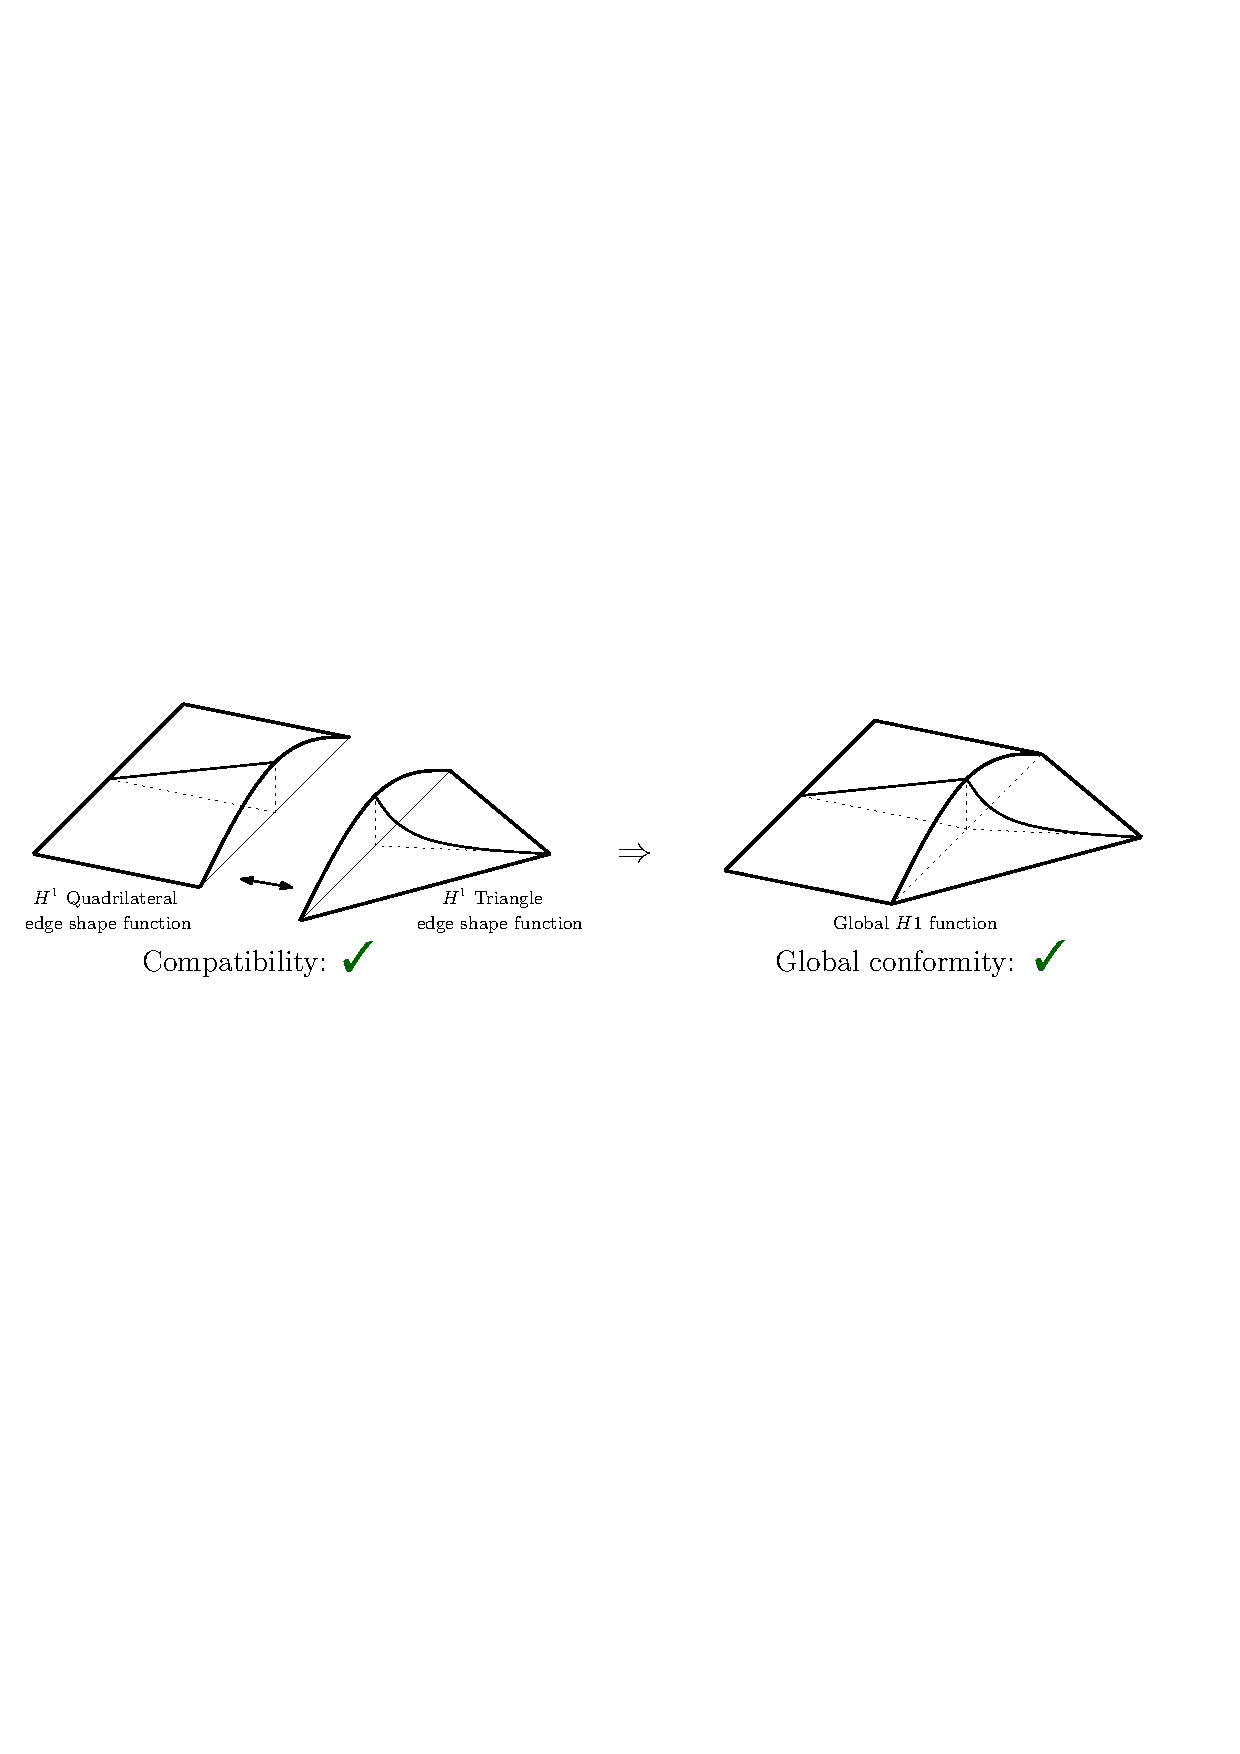
\includegraphics[scale=0.7]{./figures/CompatibilityDefinition.pdf}
\caption{Example of compatible $H^1$ edge functions resulting in a globally conforming $H^1$ function.}
\label{fig:compatibilitydefinition}
\end{center}
\end{figure}

% To be (globally) conforming to a certain energy space, shape functions of adjacent elements should be continuous at the trace level across the shared interelement boundaries.
% This is referred to as \textit{compatibility}.
% For instance, in 2D, an order $p$ edge shape function of a quadrilateral should be compatible with the order $p$ edge shape function of an adjacent triangle.
%In order for this to be possible, shape functions related to a given entity have to satisfy certain trace properties.
%The shape functions related to a given entity have to satisfy certain trace properties to ensure that they are \textit{compatible} (continuous at the trace level) with other shape functions from adjacent elements (related to the same entity).
%These properties are explained next.

\subsection{Embedded Sequences and Dimensional Hierarchy}
\label{sec:dimensionalhierarchy}

To enforce compatibility, it is useful to actually begin with a known trace over the (shared) boundary and then extend (or lift) it to the rest of the element.
This is the approach inherently present in our constructions.
In fact, this idea is reinforced when looking at the exact sequences.
%Next is a fundamental observation regarding exact sequences and the number of spatial dimensions:
Note the crucial fact that the lower dimensional sequences are ``embedded'' in the higher dimensional sequences if one considers the appropriate restrictions.
This is better represented by the following diagram,
\begin{equation}
	\begin{gathered}
  %\text{2D:}&\qquad H^1 \xrightarrow{\,\,\nabla\,\,} H(\mathrm{curl}) \xrightarrow{\nabla\times} L^2 \\
  %\text{1D:}&\qquad H^1 \xrightarrow{\,\,\nabla\,\,} L^2\,.
  	\xymatrix{
        {\text{3D:}} & H^1 \ar[r]^{\nabla\,\,\,\,} \ar@{.>}[d]^{\mathrm{tr}} & H(\mathrm{curl})
          \ar[r]^{\,\,\,\nabla\times} \ar@{.>}[d]^{\mathrm{tr}} & H(\mathrm{div})
          	\ar[r]^{\,\,\,\nabla\cdot} \ar@{.>}[d]^{\mathrm{tr}} & L^2\\
        {\text{2D:}} & H^1 \ar[r]^{\nabla\,\,\,} \ar@{.>}[d]^{\mathrm{tr}} & H(\mathrm{curl})
          \ar[r]^{\,\,\,\nabla\times} \ar@{.>}[d]^{\mathrm{tr}} & L^2\\
        {\text{1D:}} & H^1 \ar[r]^{\nabla\,\,\,\,} & \,\,\,\,L^2\,,\, }
	\end{gathered}\label{eq:traceexactsequences}
\end{equation}
where the ``mapping arrows'', $\xymatrix{{}\ar@{.>}[r]^{\mathrm{tr}}&{}}$, indicate that the range (of the trace) is actually a larger space.
These arrows are meant to be motivational only.
At the discrete level, we always reproduce the above diagram precisely with the dotted lines being replaced by well defined maps.

Indeed, we will enforce a \textit{dimensional hierarchy} through traces which is consistent with the previous discussion.
The template for this new form of hierarchy is precisely \eqref{eq:traceexactsequences}, but it is satisfied at the level of the shape functions themselves (not only the spaces).
One will begin the construction by first defining the 1D shape functions (over the segment), then defining all the 2D functions (over the quadrilateral and triangle), and finish with the 3D shape functions.
%Throughout the construction, through the trace operation, the shape functions should be nested % (e.g. the trace of a 2D $H^1$ edge function, restricted to the corresponding edge, will produce a 1D $H^1$ function).
%and therefore, all higher dimensional shape functions are actually extensions of lower dimensional ones.
Throughout the construction, the higher dimensional shape functions will have as (nonzero) trace a lower dimensional function,
so that they are actually extensions of these lower dimensional functions.
Indeed, the shape functions are nested through the trace operation at each topological entity lying in the boundary.

For example, given an edge of a 2D element, the nonzero edge traces of the 2D $H^1$ shape functions should reproduce the 1D $H^1$ shape functions.
Hence, some 2D $H^1$ shape functions are said to be extensions of the 1D $H^1$ shape functions.
Similarly, the nonzero edge trace of 2D $H(\mathrm{curl})$ shape functions should be the 1D $L^2$ shape functions (see \eqref{eq:traceexactsequences}).
These relations hold per topological entity as well.
For example, the nonzero edge trace of 2D $H^1$ \textit{vertex} functions should coincide with the 1D $H^1$ \textit{vertex} functions, and the nonzero trace of the 2D $H^1$ \textit{edge} functions should coincide with the 1D $H^1$ \textit{edge} functions (see Figures \ref{fig:2Dvertexcompatibility} and \ref{fig:2Dedgecompatibility} later on).
%The 1D trace of the 2D $H^1$ \textit{face} functions will be zero.
When enforced, these nice relationships not only aid in the compatibility, but, from the computational standpoint, have the benefit of allowing us to recycle a large amount of code when moving from one element construction to another.
%This implies, for example, that 2D $H^1$ edge functions are extensions (to the quadrilateral or triangle) of known 1D (segment) $H^1$ edge functions.
%Similarly, 2D $H(\mathrm{curl})$ edge functions are extensions of known 1D $L^2$ edge functions.
%Regarding the number of components, this is possible because the 2D $H(\mathrm{curl})$ (tangential) \textit{trace} only has one component.
%This will be clearer when the shape functions are actually constructed.

\subsection{Basic Properties of Shape Functions}

In this section we will describe the basic properties that our shape functions should satisfy.
These properties are specific to the topological entity (vertices, edges, faces, interior) and the energy space to which the shape functions are associated.
For example, vertex functions satisfy different properties than edge functions in $H^1$, and 2D edge functions satisfy different properties in $H^1$ and $H(\mathrm{curl})$.

%The number of shape functions related to a given topological entity is different.
%Generally speaking, 
For a given element and energy space, each topological entity owns a set of shape functions, which is said to be \textit{associated} to the entity.
These functions are nonzero at the associated topological entity.
Indeed, each vertex is associated to \textit{one} $H^1$ vertex shape function.
Meanwhile, each edge, face, and interior of the element is associated to a \textit{set} of edge, face, and interior shape functions of size of the order of $p$, $p^2$ and $p^3$ respectively.
%The functions are nonzero at the associated topological entity.
For example, in $H^1$, each edge is associated to a set of $p-1$ edge shape functions.
 %(and the same holds for $H(\mathrm{curl})$). 
%while each face is associated to sets of $H^1$, $H(\mathrm{curl})$ and $H(\mathrm{div})$ face shape functions, each having about $p^2$ functions.
%Moreover, for a given energy space, each edge, face, and interior of the element is associated to a \textit{set} of edge, face, and interior shape functions with size on the order of $p$, $p^2$ and $p^3$ respectively. 
%That is, there are around $p$ shape functions associated to every edge
%\footnote{Here, again we are being liberal in the use of $p$, which loosely denotes the polynomial order. In fact, $p$ is a multi-index for the quadrilateral, hexahedron and prism.}

Now, for a given dimension, space, and topological entity, we will cover three main aspects of the shape functions.
First, are the vanishing properties that they should satisfy.
These properties establish a form of trivial compatibility along some parts of the boundary.
Functions whose trace vanishes everywhere along the boundary are called \textit{bubbles}, and they are trivially compatible with each other.
Second, come the nonzero trace properties.
These are, in general, nontrivial, and ensure either full compatibility or compatibility modulo ``orientations'' (see \S\ref{sec:introorientations} for a discussion on ``orientations'').
Fortunately, dimensional hierarchy will determine the form of these nonzero traces.
Third, are some properties that the shape functions should satisfy along the element itself in order to have hierarchy in $p$.


%Throughout this description, the aspect of dimensional hierarchy through traces will be seen to be extremely practical (if not fundamental) in satisfying the compatibility of the shape functions.
%Next, we present the required trace properties, along with a more detailed view of the whole logic of the construction.
%As discussed above, the construction will enforce both the typical hierarchy in order $p$ and the dimensional hierarchy through traces.

\subsubsection{1D}

In one dimension, classification of shape functions is:
\begin{align*}
  H^1:&\quad\text{vertex and edge functions,}\\
  L^2:&\quad\text{\phantom{vertex and} edge functions.}
\end{align*}
There is only one simply connected 1D element, which is the segment (or edge), and its boundary is just its two vertices.
%Each of the (two) vertices is related to \textit{one} vertex shape function.
%The edge is associated to a set of edge functions.

\paragraph{$H^1$.}
\textit{Vertex functions:} %Consider the vertex functions.
First, there are the vanishing properties.
The vertex functions should vanish at the other (unassociated) vertex.
Second, there are the nonzero trace properties.
The vertex functions should take the value $1$ at the associated vertex.
This will ensure \textit{full} compatibility in 1D.
%This is enough to satisfy compatibility across interelement boundaries in one dimension.
Third, there is the form of the function itself.
There are multiple ways in which the vertex function can decay towards the other vertex (see Figure \ref{fig:vertexcompatibility}).
%This is referred to as \textit{vertex blending across the edge}. %, and is a concept that becomes more important when satisfying compatibility at higher spatial dimensions.
If the hierarchy in $p$ is not an issue, the decay could be nonlinear and dependent on $p$, and this may have some computational advantages.
For example, when having a mesh with uniform order $p$ across all elements, this nonlinear decay might lead to a better conditioning of finite element matrices.
%Despite this, depending on the order $p$ of the element, the blending could be chosen as nonlinear.
%This would destroy the hierarchy in $p$, but could lead to some advantages, such as better conditioning of finite element matrices.
%When having a mesh with uniform order $p$ across all elements, this could be a useful asset, but the notion of $p$ adaptivity, which requires hierarchy in $p$, is important to us.To maintain hierarchy in $p$, this decay is chosen as linear in this work.
However, as mentioned before, we want our shape functions to be useful in $p$ adaptive environments in higher dimensions.
Hence, we enforce hierarchy in $p$, and this restricts our choice to $p=1$, so the decay must be linear.
Indeed, this is the typical and simplest choice.

\begin{figure}[!ht]
\begin{center}
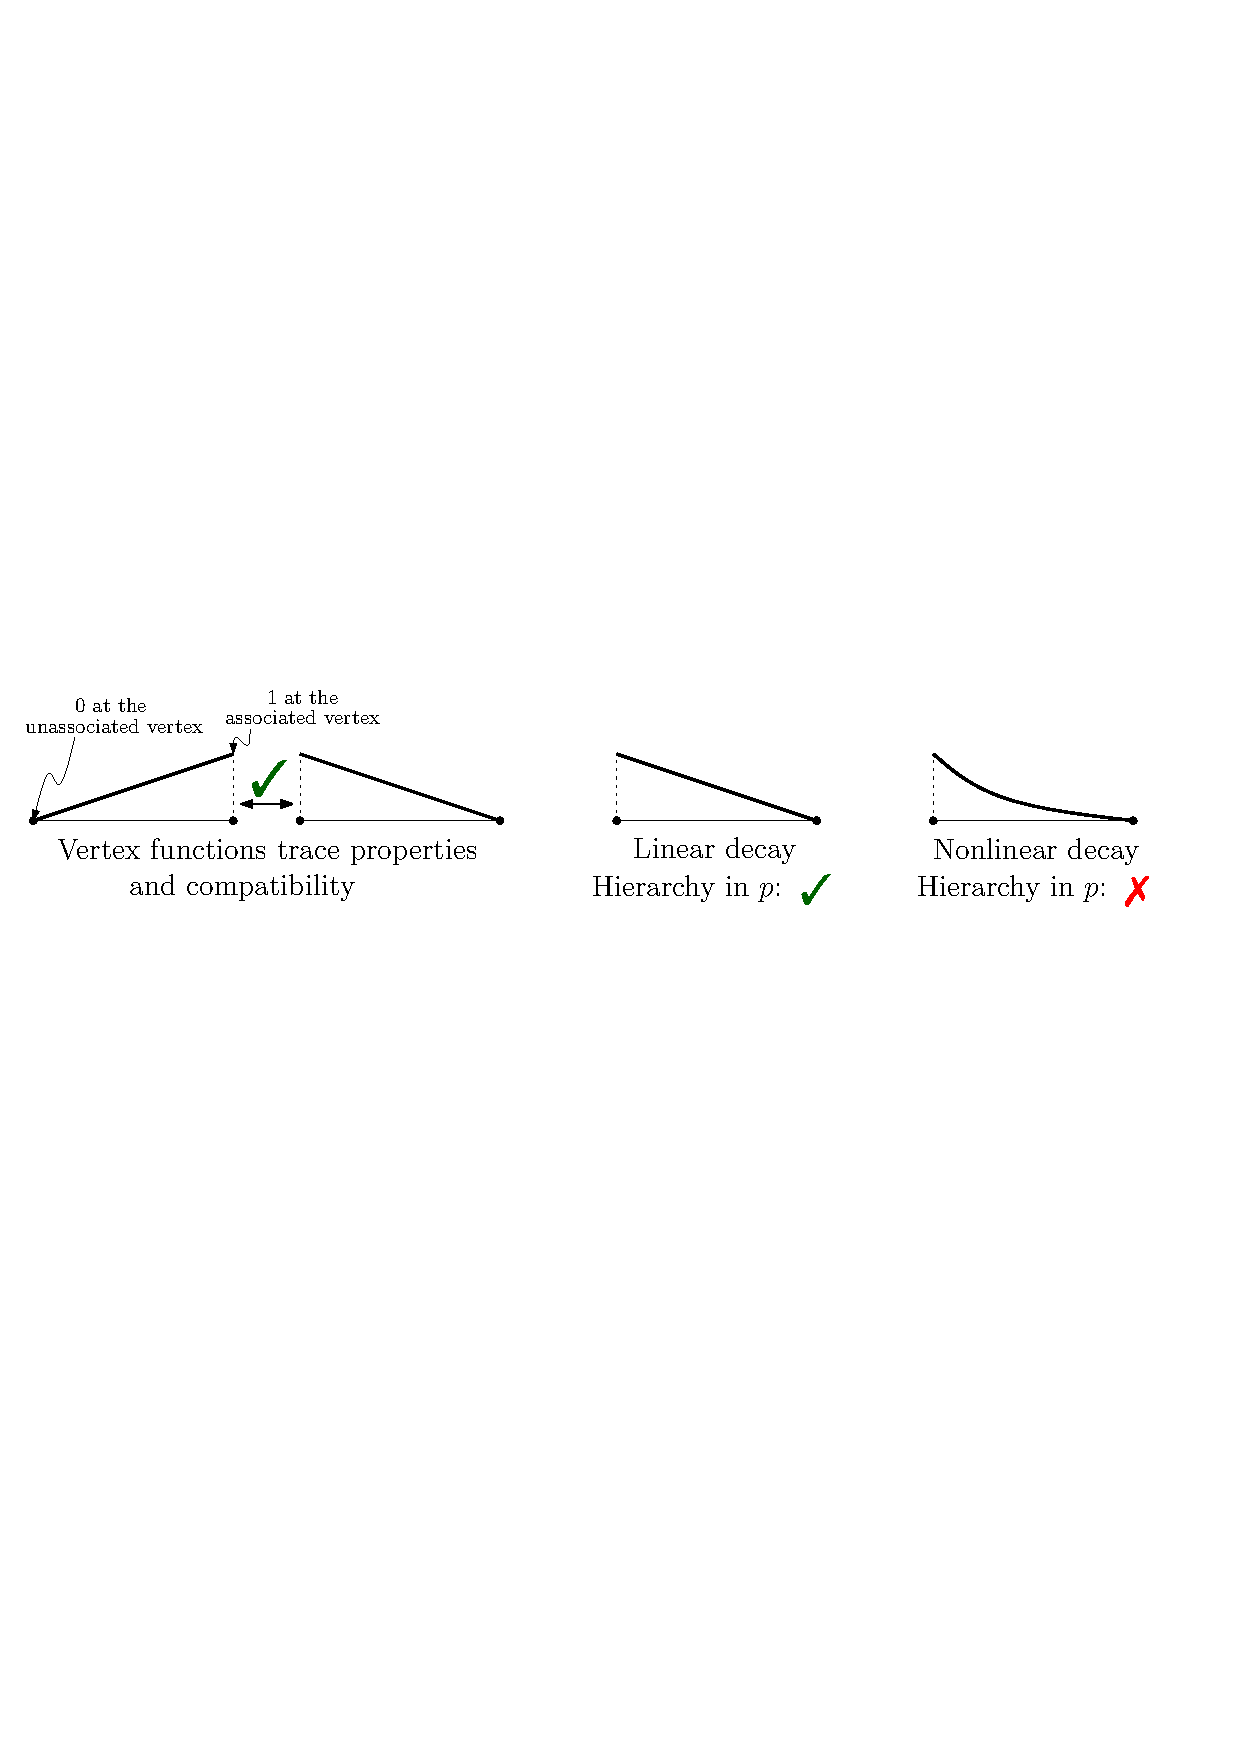
\includegraphics[scale=0.7]{./figures/VertexCompatibilityAndBlending.pdf}
\caption{Natural vertex function compatibility and the different possible decays.}
\label{fig:vertexcompatibility}
\end{center}
\end{figure}

%In general, functions which vanish at \textit{all} of the boundary are called \textit{bubbles}.
\textit{Edge functions:} In 1D the $H^1$ edge shape functions are called \textit{edge bubbles} and should vanish at the two endpoints of the edge (or segment).
This makes them automatically compatible in 1D.
When $p=1$ there are no edge bubbles, when $p=2$ there is one $p=2$ edge bubble, when $p=3$ there is the $p=2$ bubble and an extra $p=3$ bubble giving a total of two bubbles, and so on.
This results in a hierarchical construction of the shape functions in $p$.
%These hierarchically constructed edge bubbles will constitute the group of edge shape functions.
%They are referred to as \textit{the} 1D $H^1$ edge bubbles.

%Due to the dimensional hierarchy, the 1D trace of $H^1$ vertex and edge functions of elements in higher dimensions (quadrilateral, triangle, hexahedron, etc.) will be precisely the 1D $H^1$ vertex and edge functions.
%This is important, because as evidenced by \eqref{eq:traceexactsequences}, the trace of $H^1$ edge functions of elements in higher dimensions (quadrilateral, triangle, hexahedron, etc.) will be exactly one of \textit{the} 1D $H^1$ edge bubbles (modulo an orientation).

\begin{figure}[!ht]
\begin{center}
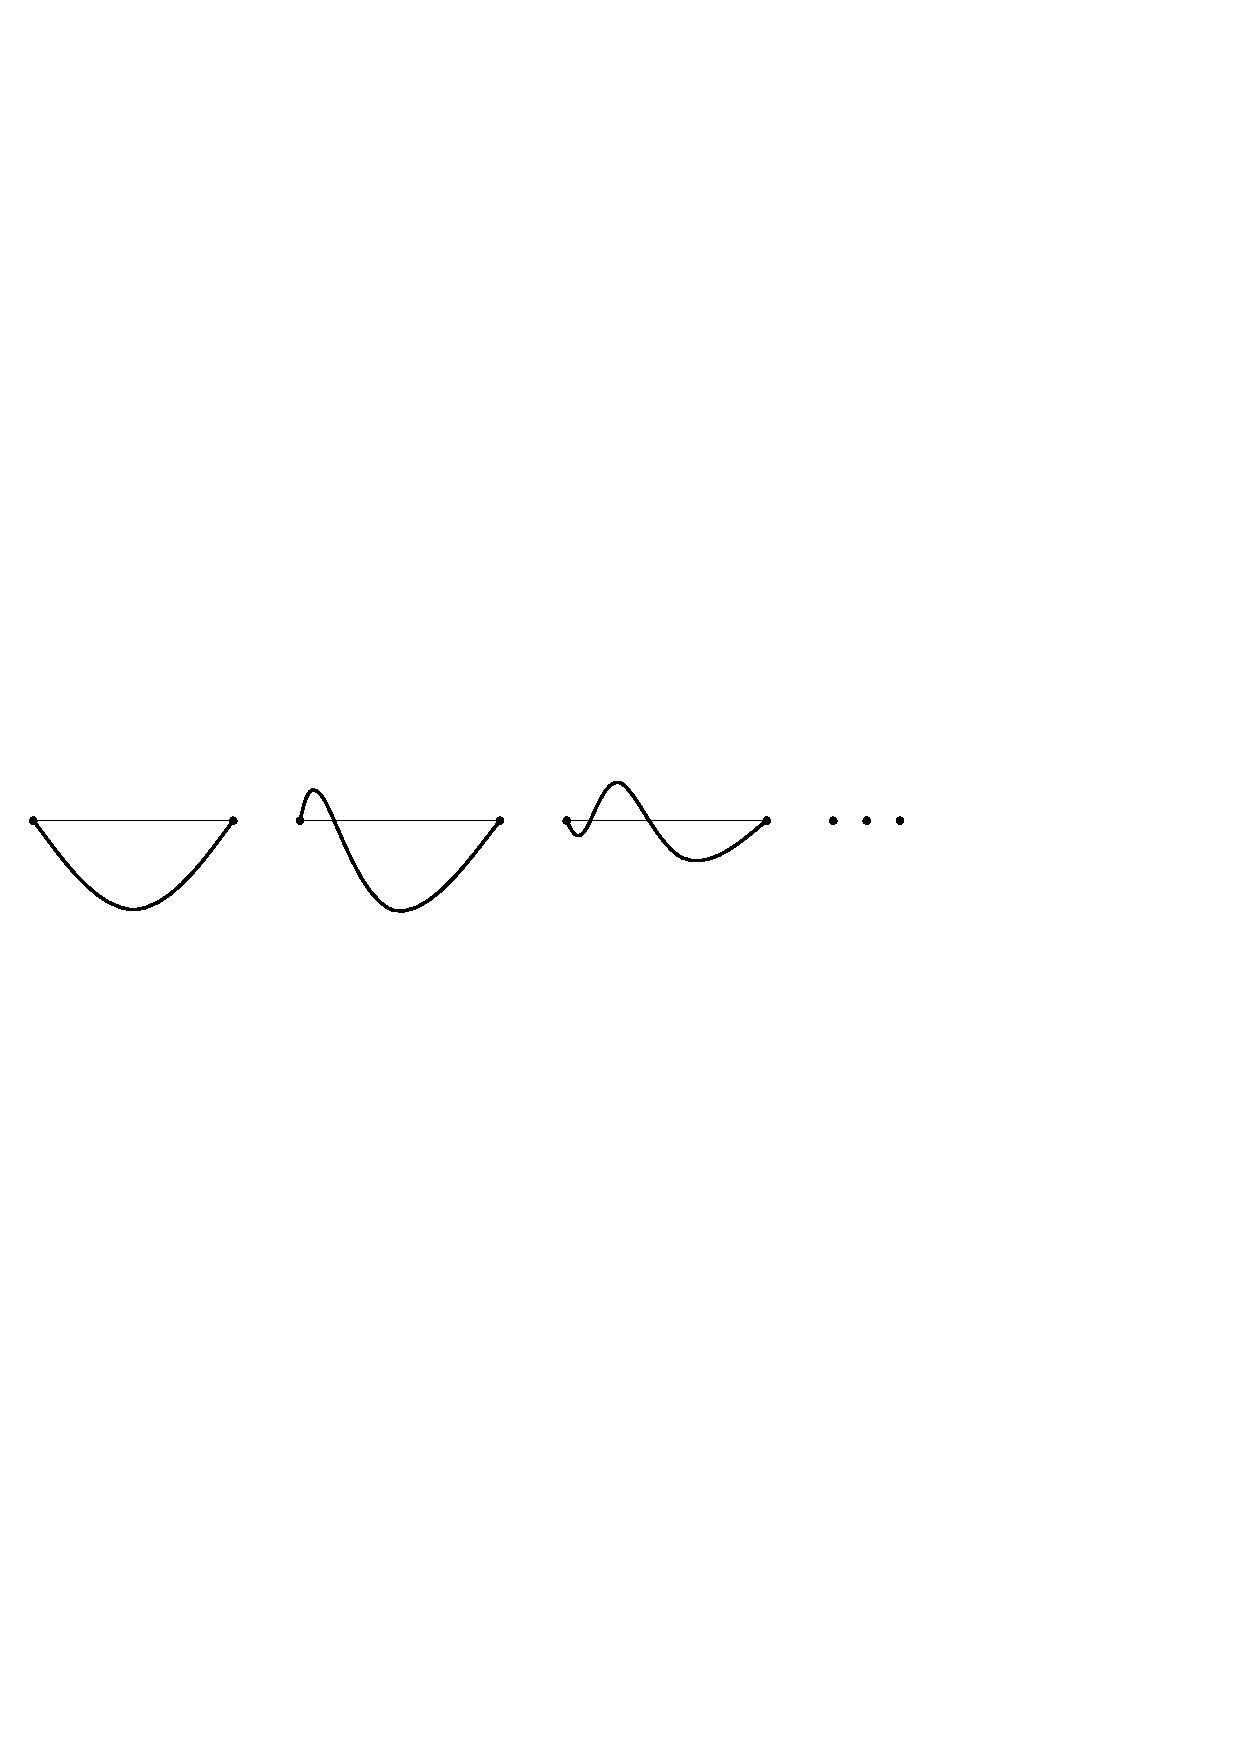
\includegraphics[scale=0.7]{./figures/H1Bubbles.pdf}
\caption{Potential set of of 1D $H^1$ edge bubbles vanishing at both endpoints.}
\label{fig:1DH1bubbles}
\end{center}
\end{figure}

\paragraph{$L^2$.}
\textit{Edge functions:}
The 1D $L^2$ edge functions do not need to satisfy any trace properties (neither vanishing nor nonzero) because there is no notion of trace.
They span the space of the (1D) gradients of the $H^1$ conforming shape functions, and should be hierarchical in their construction.
%They are referred to as \textit{the} 1D $L^2$ edge functions.

\subsubsection{2D}

In two dimensions, classification of shape functions is:
\begin{align*}
  	H^1:&\quad\text{vertex, edge, and face functions,}\\
  	H(\mathrm{curl}):&\quad\text{\phantom{vertex,} edge, and face functions,}\\
  	L^2:&\quad\text{\phantom{vertex, edge, and} face functions.}
\end{align*}
There are two 2D elements: the quadrilateral and the triangle.
Their boundaries are composed of edges and vertices.
%For a given element, each vertex is related to \textit{one} vertex shape function, each edge is associated to a set of edge funtions, and the face is associated to a set of face functions.
%The edge is associated to a set of edge functions.

\paragraph{$H^1$.}
\textit{Vertex functions:}
The vertex functions should vanish at the other (unassociated) vertices and disjoint edges.
They should take the value $1$ at the associated vertex.
In 2D, at this point, this does \textit{not} guarantee compatibility.
However, dimensional hierarchy requires the (nonzero) trace of vertex functions over the adjacent edges to be precisely a 1D $H^1$ vertex function (associated to the vertex in question).
This results in full compatibility, and implies the 2D vertex functions are extensions of their 1D analogues.
%Here, one additionally has to ensure that the trace  always presents the same decay.
%For example, see Figure \ref{fig:2Dvertexcompatibility} (right) for a pair of vertex shape functions satisfying the correct vanishing properties, but being incompatible due to the different decay across the edges.
%If dimensional hierarchy is used, the form of this decay is fixed, since it should
%In this case, compatibility across the boundary would be automatically satisfied (see left of Figure \ref{fig:2Dvertexcompatibility}).
%Fortunately, the
%This is the choice in our work.
%Third, there is the form of the vertex functions themselves along the 2D face (quadrilateral or triangle).
Regarding the form of the shape functions across the (quadrilateral or triangle) face itself, they can have different forms of decay.
Again, hierarchy in $p$ will restrict our choice, so that the vertex functions we define lie in the lowest order space possible.
Indeed, quadrilateral vertex functions present a bilinear decay, while the decay is linear for triangles.
% This form will be quite restrictive in o
%Otherwise, to satisfy compatibility, one would have to ensure that the trace of vertex functions (for both quadrilateral and triangle) over the edges always presents the same decay.
%To ensure compatibility across edges, it is required that the trace of the vertex functions over the (adjacent) edges presents the same decay regardless of the element type (quadrilateral or triangle).
%This is automatically ensured as long as the nonzero (1D) trace of these functions along each edge is a 1D $H^1$ vertex function.
%That is, the \textit{vertex blending across the edge} should be the same for all edges of the quadrilateral and triangle.
%Notice, there is a (partly induced) \textit{vertex blending across the quadrilateral $($or triangular$)$ face}.
%Again, this choice is restricted by the hierarchy, so in this work it is chosen as bilinear for quadrilaterals and linear for triangles.
%which at this point does not affect compatibility, but it will in three dimensions.
%Again, in this work this blending will be provided by a linear function.

\begin{figure}[!ht]
\begin{center}
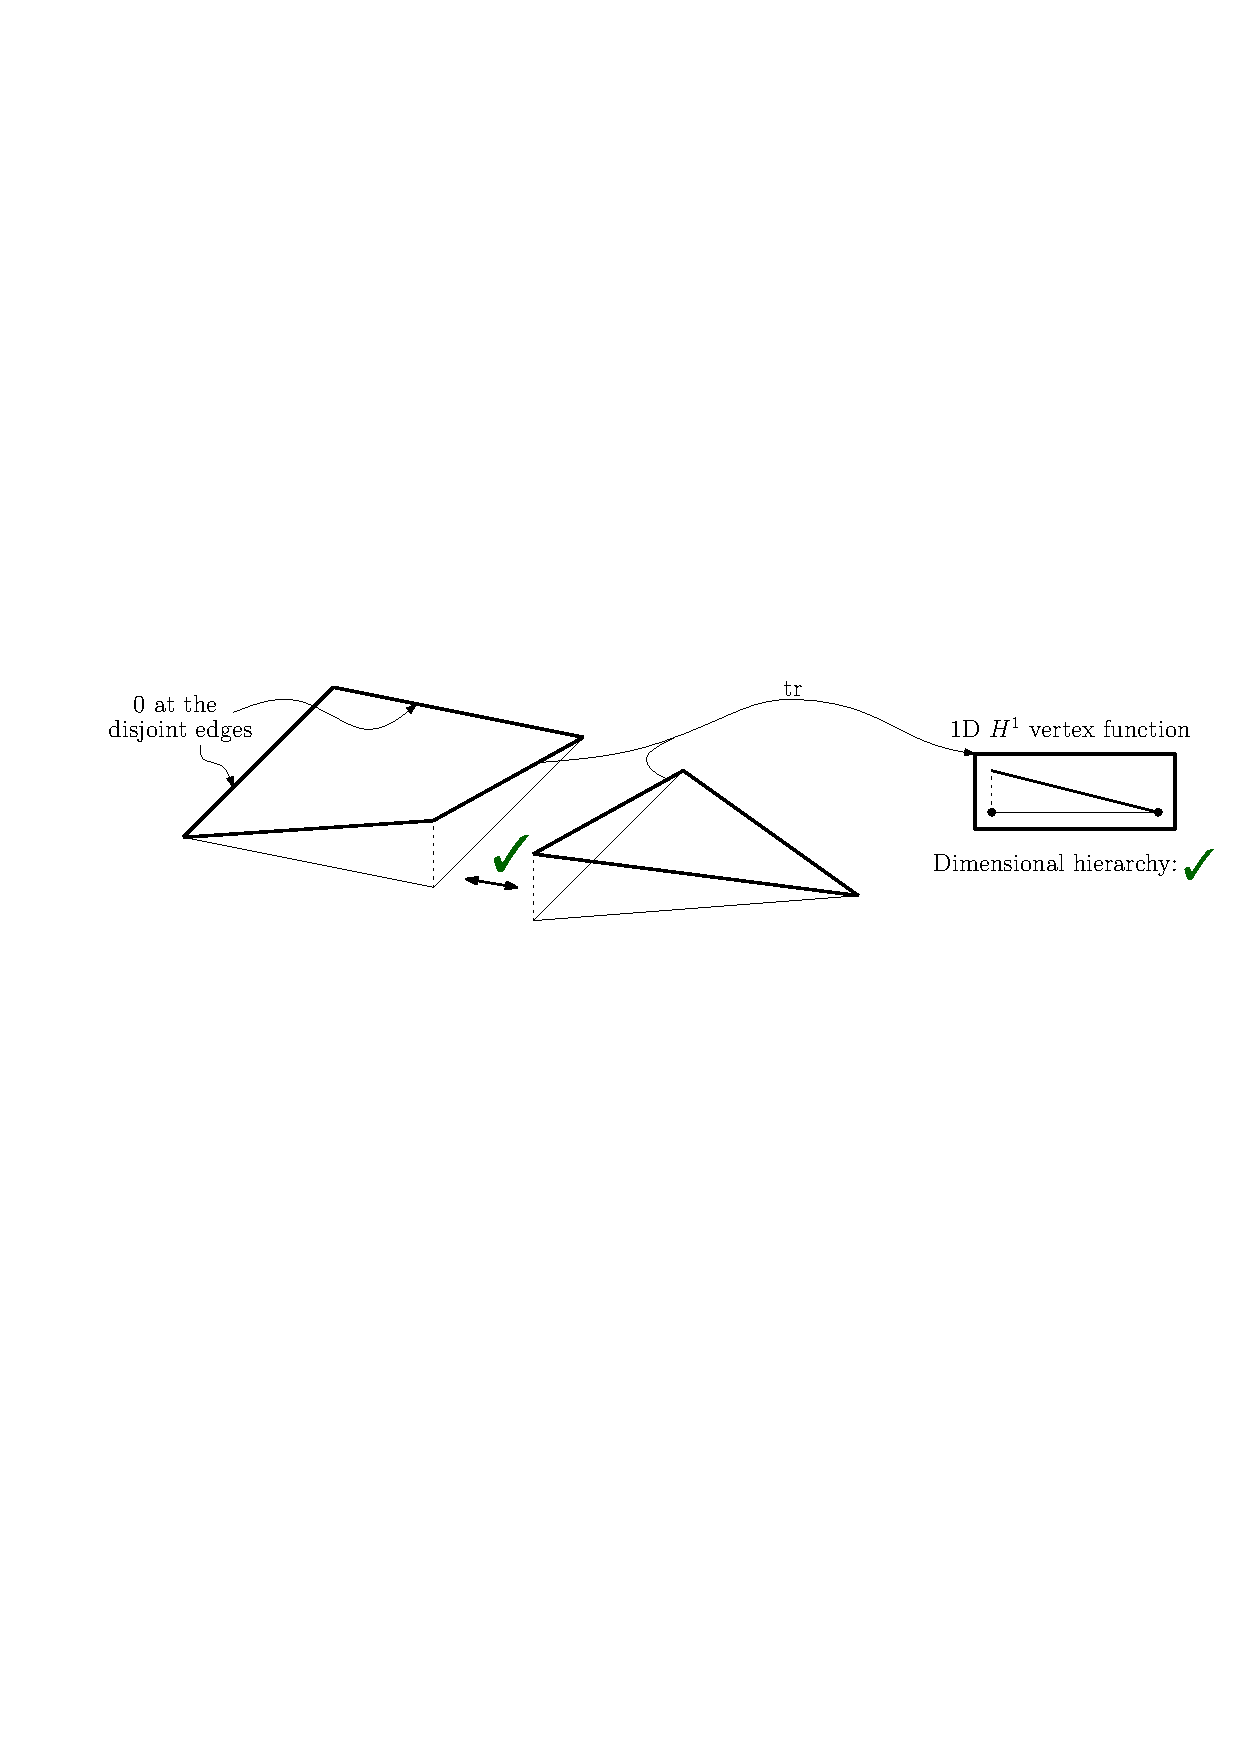
\includegraphics[scale=0.7]{./figures/2DVertexFunctions.pdf}
\caption{Trace properties of 2D $H^1$ vertex functions. Dimensional hierarchy implies full compatibility.}
\label{fig:2Dvertexcompatibility}
\end{center}
\end{figure}

\textit{Edge functions:}
Edge functions should vanish at all other (unassociated) edges of the element.
By dimensional hierarchy, for a given order $p$, the nonzero trace over the (associated) edge itself should take the form of a 1D $H^1$ edge bubble of order $p$.
This gives compatibility modulo edge ``orientations'' in 2D, and it implies the edge functions are extensions of the original 1D $H^1$ edge bubbles.
%All edge shape functions (of a given order $p$) should present the same nonzero trace over the (associated) edge itself.
%Indeed, by \eqref{eq:traceexactsequences} and by dimensional hierarchy, if the trace of the edge functions are the 1D $H^1$ edge bubbles, then compatibility modulo ``orientations'' is satisfied.
%In view of the embeddings shown in \eqref{eq:traceexactsequences}, it follows that at the edge itself the function is one of \textit{the} 1D $H^1$ edge bubbles (the ones coming from the 1D element).
%This is enough to ensure compatibility (modulo orientations) across the boundaries.
%This would imply the edge functions are extensions of the original 1D $H^1$ edge bubbles.
%The extension to the rest of the element involves satisfying the vanishing properties at the other edges, meaning that the function has to somehow decay.
Now, the functions themselves should present a certain decay from the (associated) edge towards the rest of the element.
%This decay is referred to as \textit{edge blending across the quadrilateral $($or triangular$)$ face}.
Again, this choice is generally restricted by the hierarchy in $p$.
For the quadrilateral element the decay we invoke is linear, but things are more complicated for the triangle element. %where the order of decay depends upon the order of the edge function.
%This affects compatibility of the edge functions only in 3D.

\begin{figure}[!ht]
\begin{center}
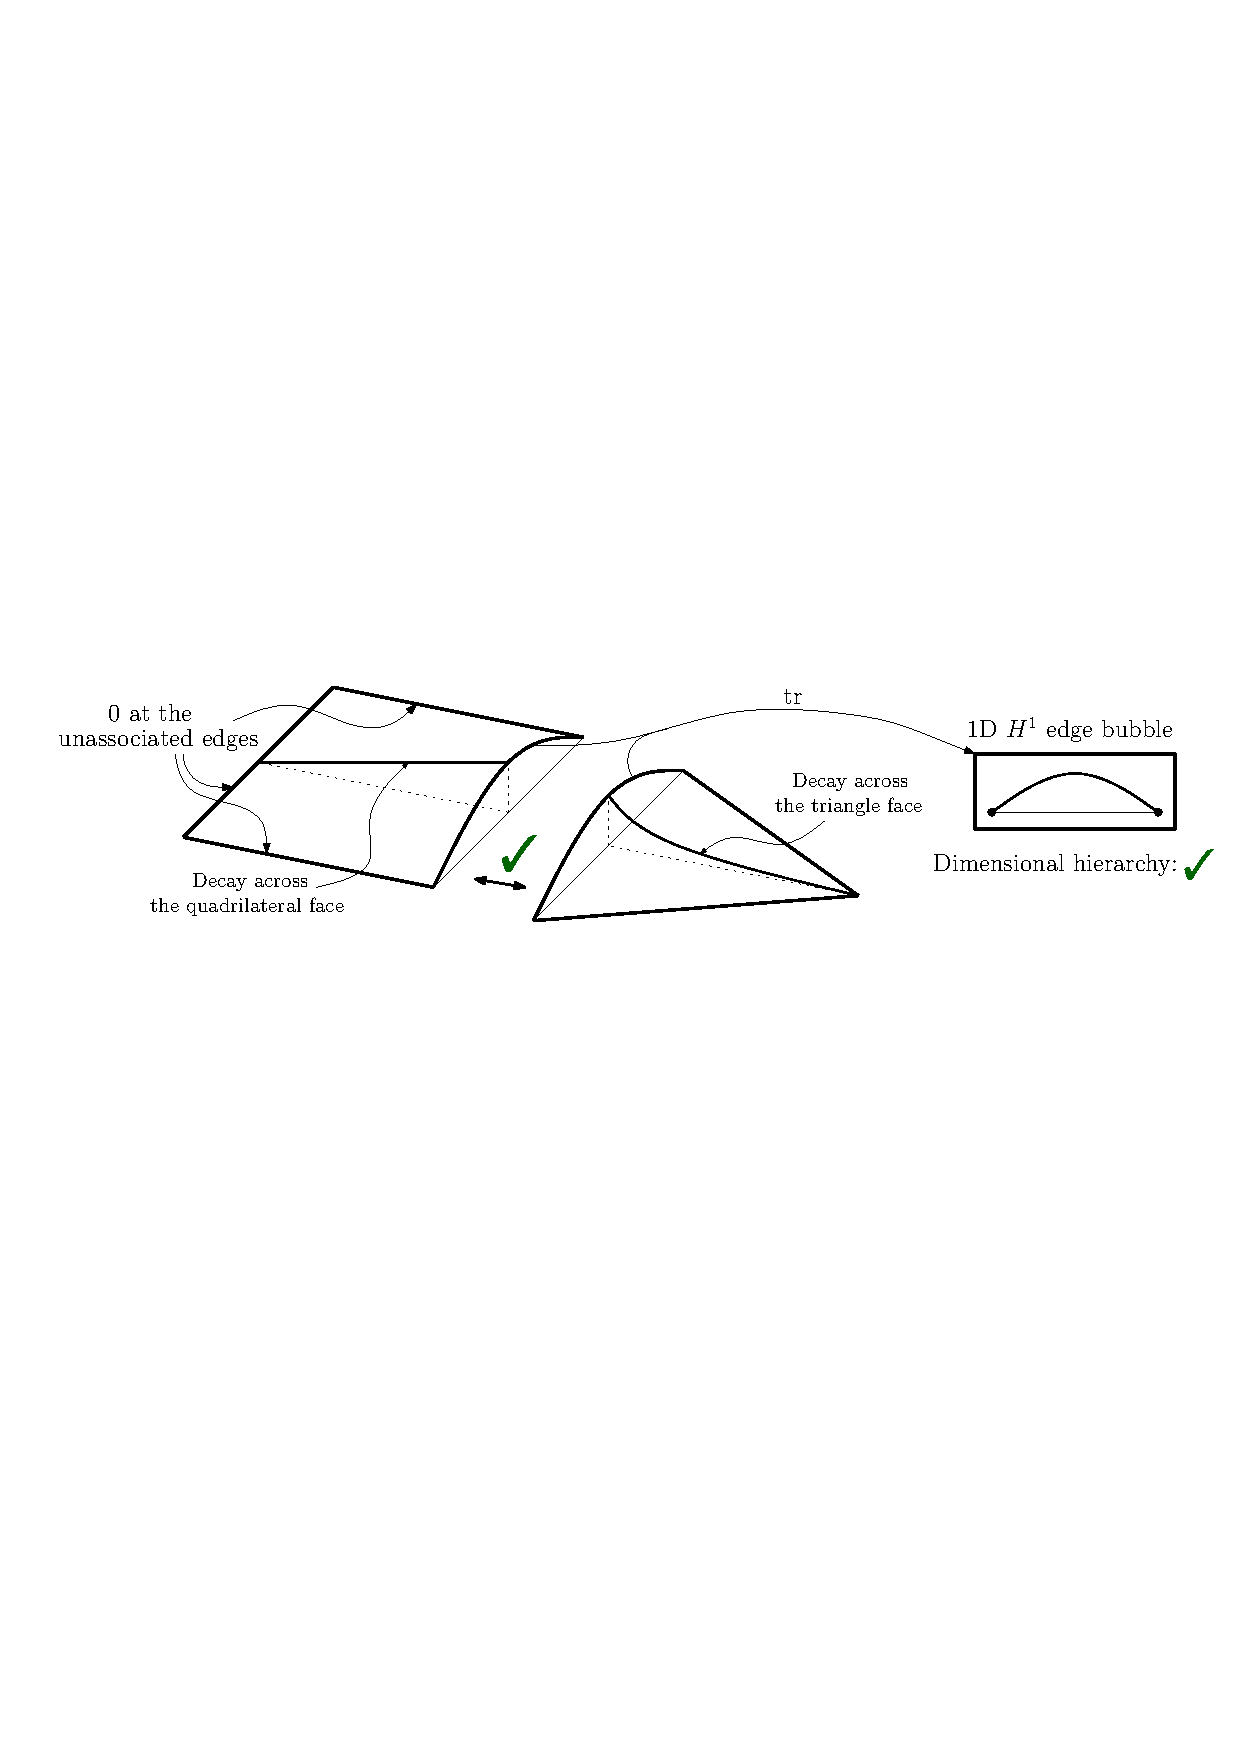
\includegraphics[scale=0.7]{./figures/EdgeBlendingQuadTri.pdf}
\caption{Compatibility of edge functions. Depicted as well is the decay across the faces.}
\label{fig:2Dedgecompatibility}
\end{center}
\end{figure}

\textit{Face functions:}
The 2D \textit{face bubbles} vanish at all the edges of the element, so they are automatically compatible in 2D.
They are constructed usually by using the edge functions previously defined (since these already satisfy some vanishing properties) and making some modifications to establish the remaining vanishing conditions.
Again, their construction is hierarchical in $p$.
%The resulting functions are said to be \textit{the} 2D $H^1$ quadrilateral (or triangle) face bubbles.

\paragraph{$H(\mathrm{curl})$.}
\textit{Edge functions:}
The edge functions must have vanishing (tangential) trace at all other edges.
For a given order $p$, the nonzero (tangential) trace over the edge itself should take the form of a 1D $L^2$ edge function of order $p$.
This ensures compatibility modulo edge ``orientations''.
%Meanwhile, the (tangential) trace of the edge functions (of order $p$) over the edge itself (which has one component) should be the same.
%By dimensional hierarchy (see \eqref{eq:traceexactsequences}), if they are chosen as the 1D $L^2$ edge functions, full compatibility is ensured.
Now, to respect hierarchy in $p$, the edge functions themselves should present a decay (in each of their two components) which is consistent with the lowest order possible decay.
Ultimately, the decay will be similar to that of $H^1$ edge functions.

\textit{Face functions:}
The face bubbles have zero (tangential) trace over all edges, so they are automatically compatible.
They are hierarchically constructed using the same ideas as for their $H^1$ counterparts.
%They are said to be \textit{the} 2D $H(\mathrm{curl})$ quadrilateral (or triangle) face bubbles.

\paragraph{$L^2$.}
\textit{Face functions:}
The $L^2$ face functions do not need to satisfy any trace properties, because there is no notion of trace in $L^2$.
They span the space of (2D) curls of the $H(\mathrm{curl})$ shape functions, and their construction should be hierarchical in $p$.
%and are said to be \textit{the} 2D $L^2$ quadrilateral (or triangle) face functions.

\subsubsection{3D}

In three dimensions, classification of shape functions is:
\begin{align*}
  H^1:&\quad\text{vertex, edge, face, and interior shape functions,}\\
  H(\mathrm{curl}):&\quad \text{\phantom{vertex,} edge, face, and interior shape functions,}\\
  H(\mathrm{div}): &\quad\text{\phantom{vertex, edge,} face, and interior shape functions,}\\
  L^2:&\quad\text{\phantom{vertex, edge, face, and} interior shape functions.}
\end{align*}
There are four 3D elements: the hexahedron, the tetrahedron, the prism and the pyramid.
Their boundaries are composed of faces, edges, and vertices.
%For a given element, each vertex is related to \textit{one} vertex shape function, each edge is associated to a set of edge funtions, each face is associated to a set of face functions, and the interior is associated to a set of interior functions.


\paragraph{$H^1$.}
\textit{Vertex functions:}
Vertex functions have to vanish at all other (unassociated) vertices and at all disjoint edges and faces.
Dimensional hierarchy requires the (nonzero) trace of vertex functions over the adjacent faces to be precisely a 2D $H^1$ vertex function (associated to the vertex in question).
This ensures full compatibility of the vertex functions in 3D.
%The decay of the functions across edges \textit{and} faces should be the same in order to enforce compatibility.
%Hence, the vertex functions of all elements should present the same nonzero vertex blending across the edges.
%The same goes for the vertex blending across quadrilateral and triangular faces.

\textit{Edge functions:}
Edge shape functions should vanish at all other (unassociated) edges and disjoint faces.
By dimensional hierarchy, for a given order $p$, the nonzero trace over the adjacent faces should be a 2D $H^1$ edge function of order $p$ (associated to the edge in question).
Again, this ensures compatibility modulo edge ``orientations''.
%Again, the trace of functions at the edge itself must be one of \textit{the} 1D $H^1$ edge bubbles, so they are 3D extensions of the original 1D function.
%To ensure compatibility (modulo orientations), the functions should have the same \textit{edge} blending across the quadrilateral faces and the triangular faces.

\textit{Face functions:}
Face functions should vanish at all other (unassociated) faces.
Dimensional hierarchy establishes that, for a given order, the nonzero trace over the (associated) face itself should be a 2D $H^1$ face bubble of the same order.
This establishes compatibility modulo face ``orientations''.

\textit{Interior functions:}
The 3D \textit{interior bubbles} vanish at all faces of the element, and are fully compatible in 3D.
Our construction of these functions usually involves making some changes to the face functions previously defined in order to establish the remaining vanishing conditions.

\paragraph{$H(\mathrm{curl})$.}
\textit{Edge functions:}
The edge functions must have vanishing (tangential) trace at all other edges and disjoint faces.
For a given order $p$, the nonzero trace over the adjacent faces should be a 2D $H(\mathrm{curl})$ edge function of order $p$.
This gives compatibility modulo edge ``orientations''.
%As mentioned before the (tangential) trace of the edge function over the edge itself (which has one component) must be one of \textit{the} 1D $L^2$ edge functions.
%For compatibility, the \textit{edge} blending across the quadrilateral faces and the triangular faces should be the same.

\textit{Face functions:}
The face functions have vanishing (tangential) trace over all other faces.
%Using \eqref{eq:traceexactsequences} it is clear that the (tangential) trace over the face must be one of \textit{the} 2D $H(\mathrm{curl})$ quadrilateral or triangle face bubbles.
Requiring the trace over the face itself to be a 2D $H(\mathrm{curl})$ face bubble of a given order ensures compatibility modulo face ``orientations''.

\textit{Interior functions:}
The interior bubbles have zero (tangential) trace over all the faces and are fully compatible in 3D.
They are constructed using the same ideas as for interior bubbles in $H^1$.

\paragraph{$H(\mathrm{div})$.}
%In this space, there are no vertex or edge functions.
\textit{Face functions:}
The face functions should have vanishing (normal) trace at all other faces.
The trace over the face itself should be a 2D $L^2$ face function of a given order.
%Due to \eqref{eq:traceexactsequences}, they will be extensions of 2D $L^2$ face functions, and their normal component along the face should be one of \textit{the} 2D $L^2$ quadrilateral or triangle face functions.
Compatibility modulo face ``orientations'' is then established.

\textit{Interior functions:}
The interior bubbles have zero normal component at all the faces, and they are automatically compatible.
They are constructed using the same ideas as in $H^1$.

\paragraph{$L^2$.}
\textit{Interior functions:}
These do not have to satisfy any trace properties and they span the space of the (3D) divergences of the $H(\mathrm{div})$ shape functions.

% We shall always identify the discrete spaces first, and only then introduce the corresponding shape functions that provide bases for those spaces. It is in place perhaps to recall two competing schools of thought when it comes to the concept of shape functions.

% The classical definition of Ciarlet \cite{Ciarlet} starts with {\em degrees-of-freedom} that are functionals defined on a larger space $\mathcal{X}(\Omega)$ that contains both the space of element shape functions
% $X(\Omega)$  and the exact solution,
% $$
% \psi_j : \mathcal{X}(\Omega) \to \mathbb{R}, \quad j=1,\ldots, N_\Omega \, .
% $$
% Here, $N_\Omega$ denotes the number of degrees of freedom. In this definition,the condition of {\em unisolvability} is critical; the restrictions, $\psi_j\vert_{X(\Omega)}$, must provide a basis for the algebraic dual space $X(\Omega)^\ast$. The element shape functions $\phi_i$ are defined then as the {\em dual basis} to the degrees-of-freedom,
% $$
% \psi_j(\phi_i) = \delta_{ij},\quad i,j=1,\ldots,N_\Omega \, .
% $$
% This naturally leads to the definition of the {\em interpolation operator}:
% $$
% \Pi : \mathcal{X}(\Omega) \ni u \to \Pi u := \sum_{j=1}^{N_\Omega} \psi_j(u) \phi_j \in X(\Omega) \,  .
% $$
% A judicious choice of degrees-of-freedom must guarantee {\em global conformity}, i.e. by ``gluing'' (taking unions of) shape functions, global Galerkin {\em basis functions} are constructed which belong to the appropriate energy spaces. Global conformity depends  upon the energy space. For instance, $H^1$-conforming shape functions must be globally continuous while the vector-valued $H(\text{curl})$-conforming shape functions must only be continuous in their tangential components across interelement boundaries. Similarly, for vector-valued $H(\text{div})$-conforming shape functions, only the continuity of only the normal component is enforced. Finally, $L^2$-conformity does not involve any continuity assumptions at all.

% Different energy spaces also lead to different notion of {\em traces}. By the $H^1$ trace of a scalar-valued (sufficiently) regular function, we understand simply its restriction to the boundary. By the (tangential) $H(\text{curl})$ trace of a vector-valued function, we understand the restriction of its {\em tangential component} on the boundary. Thus, the  $H(\text{curl})$ trace of a two component function $(E_1,E_2)$ in $\mathbb{R}^2$ to an element edge, is going to be a scalar-valued function. In 3D, however, the trace of a 3D vector-valued function to an element face, will be a 2D vector. Similarly, the (normal) $H(\text{div})$ trace of a vector-valued function to an edge (2D) or a face (3D) is always a vector orthogonal to the element boundary that involves
% just one scalar component.

% Global conformity considerations lead naturally to the classification of degrees-of-freedom and also naturally distributes the shape functions into groups related to geometric entities:
% $$
% \begin{array}{rl}
%   H^1:& \text{vertex, edge, face, and interior shape functions,}\\
%   H(\text{curl}):& \text{\phantom{vertex,} edge, face, and interior shape functions,}\\
%   H(\text{div}): & \text{\phantom{vertex, edge,} face, and interior shape functions,}\\
%   L^2:  & \text{\phantom{vertex, edge, face, and} interior shape functions.}
% \end{array}
% $$
% When following the Ciarlet construction, we must precompute the shape functions in terms of (usually) combinations of monomials and store the corresponding coefficients.


% The competing approach of Szabo \cite{SzaboBabuska91} starts with a direct construction of shape functions by following the geometric classification above. The shape functions are defined in terms of Legendre and Jacobi polynomials and their integrals, and are computed using simple recursive formulas. This is the approach taken in this work. Note that, in Szabo's approach, we do not define the interpolation operators at this point at all. The so-called {\em projection-based interpolation} \cite{hpbook,hpbook2} defined through local projections over element edges, faces and interior, is introduced {\em independently} of the construction of shape functions. With no need to precompute coefficients defining  the shape functions, following Szabo's approach is perhaps more convenient.

%The geometric definition of shape functions implies the corresponding {\em vanishing properties}. For instance, an $H^1$ vertex shape function corresponding to a particular vertex is unity at that vertex and vanishes at all remaining vertices. An edge shape function will be non-zero along a particular edge but it will vanish along all remaining edges. A similar property holds for the face shape functions. The trace of interior shape functions ({\em element bubbles}) will vanish on the entire element boundary and so the corresponding basis functions will be supported over the element only. Debugging of shape function routines starts usually with verification of the appropriate vanishing properties.

%\subsection{Complying with the exact sequence structure}
%\label{sec:exactsequenceembeddings}
%Construction of element shape functions should comply with the logic of 1D and 2D exact sequences for traces of element shape functions to edges and faces \cite{Schoeberl_Zaglmayr_05}. This is to a certain extent satisfied automatically in our constructions as {\em we begin} with 1D edge or 2D face shape functions defined on edges or faces and only later extend them to the element. The extensions comply with the logic of exact sequences in the sense that the ultimate 3D edge or face functions utilize only the information provided by the 1D edge or 2D face routines. For instance, construction of $H(\text{curl})$ shape functions begin with a 1D $L^2$ shape function defined along the edge that constitutes the tangential components (along the edge) of the corresponding 2D or 3D shape function. The 1D $L^2$ shape functions come with no derivative. Consequently, the computation of the curl of 2D or 3D extension must not involve such a derivative either. In the same way, an $H(\text{curl})$ face shape function should use only the tangential trace and its surface curl on the corresponding face, and the $H(\text{div})$ shape functions should use only the values of their normal components on the face.
%
%We illustrate this affinity to the exact sequence at the trace level with the following diagram applying to a 3D element:
%\begin{displaymath}
%  %\text{2D:}&\qquad H^1 \xrightarrow{\,\,\nabla\,\,} H(\mathrm{curl}) \xrightarrow{\nabla\times} L^2 \\
%  %\text{1D:}&\qquad H^1 \xrightarrow{\,\,\nabla\,\,} L^2\,.
%  \xymatrix{
%        {\text{Interior:}} & H^1 \ar[r]^{\nabla\,\,\,\,} \ar@{.>}[d]^{\mathrm{tr}} & H(\mathrm{curl})
%          \ar[r]^{\,\,\,\nabla\times} \ar@{.>}[d]^{\mathrm{tr}} & H(\mathrm{div}) \ar[r]^{\,\,\,\nabla\cdot} \ar@{.>}[d]^{\mathrm{tr}} & L^2\\
%        {\text{Face:}} & H^1 \ar[r]^{\nabla\,\,\,} \ar@{.>}[d]^{\mathrm{tr}} & H(\mathrm{curl})
%          \ar[r]^{\,\,\,\nabla\times} \ar@{.>}[d]^{\mathrm{tr}} & L^2\\
%        {\text{Edge:}} & H^1 \ar[r]^{\nabla\,\,\,\,} & \,\,\,\,L^2\,\, }\,.
%\end{displaymath}
%Here, the ``mapping arrows,'' $\xymatrix{{}\ar@{.>}[r]^{\mathrm{tr}}&{}},$ indicate that the range is actually a larger space. These arrows are meant to be motivational only.
%% For example, this suggests that the traces of discrete $H(\mathrm{div})$ functions should be in a two dimensional $L^2$ space.
%% For the polynomial spaces, this means the face functions should involve traces which are products of Legendre polynomials $P_i$.
%% Moreover, they should go in the normal component to the face.
%At the discrete level, we reproduce the above diagram precisely with the dotted lines being replaced by well-defined maps. One benefit in this approach is that it allows for a large degree of portability of code from one element construction to another.
%% Indeed we acheive this.
%
%The second aspect of the exact sequence philosophy is a careful choice of discrete energy spaces. In our discrete exact sequences for the triangle and tetrahedral elements, we use the well known $H(\text{curl})$-conforming \Nedelec~and $H(\text{div})$-conforming Raviart-Thomas spaces.\footnote{See definitions for these spaces in \S~\ref{sec:Tri} and \S~\ref{sec:Tet}.} Unlike other higher order discete energy spaces used in the literature, these spaces happen to be affine invariant while also preserving a commuting exact sequence structure. In fact, we make the distinction that all of our discrete exact sequences preserve a commuting exact sequence stucture which then ensures interpolation estimates for all of our energy spaces. \textit{cite}

\subsection{Orientation Embedded Shape Functions}
\label{sec:introorientations}

\begin{figure}[!ht]
\begin{center}
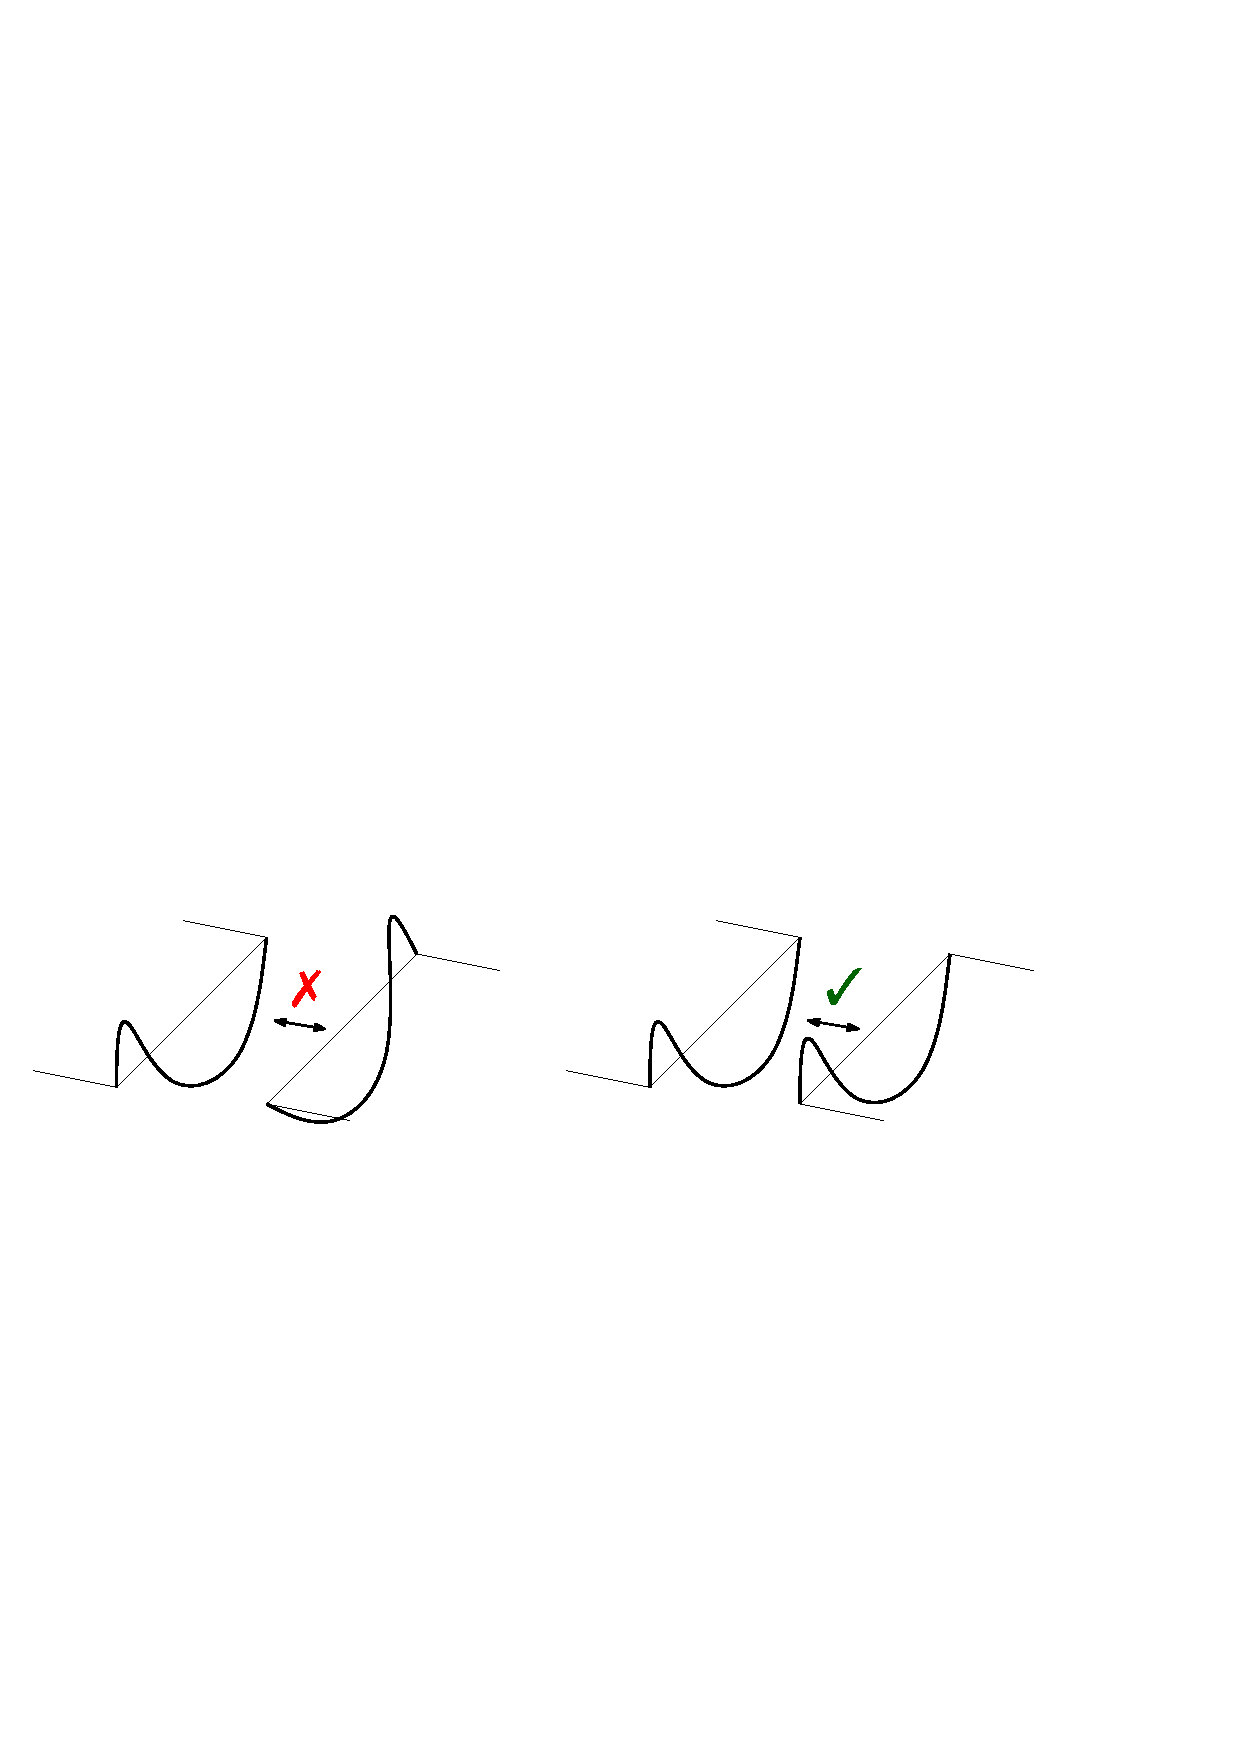
\includegraphics[scale=0.7]{./figures/OrientationsEdgeMismatch.pdf}
\caption{Potential edge function ``orientation'' mismatch in 2D due to disregarding the global mesh.}
\label{fig:edgemismatchintro}
\end{center}
\end{figure}

To ensure \textit{full} compatibility of the shape functions along the boundaries, the concept of \textit{orientations} needs to be introduced.
The simplest example occurs in 2D, where edge functions might not match in the \textit{global} mesh due to a simple change in coordinates over the edge itself.
This ``orientation'' mismatch occurs when the edge functions in the (local) master element are transformed to the global mesh.
Indeed, in the standard Szab\'o's approach, master element shape functions are constructed with no regard for global edge or face coordinates, and element shape functions contributing to an edge or face basis function may not coincide with each other along the shared boundary.
This leads to the necessity of an additional action during the finite element assembly process to account for local-to-global orientation changes (change of coordinates).
Usually, these involve \textit{sign factors} in the case of edges and quadrilateral faces, and more complicated adjustments in the case of triangle faces (see the discussion in \citet[p.50]{hpbook2}).
In the context of $h$ adaptive codes involving hanging nodes, the implementation of these modifications in the assembly procedure can become quite involved, and alternative solutions to this problem are therefore desired.

One such solution involves the concept of orientation embedding \citep{GattoDemkowicz10}.
Here, a given topological entity (an edge in 2D, or a face or edge in 3D), regardless of what elements it is adjacent to, is given a \textit{global orientation} at the mesh level, so that it effectively owns a system of coordinates.
In the mesh, this is equivalent to ordering the vertices in a certain order for that given topological entity.
For instance, for an edge with vertices $a$ and $b$, the vertices can be ordered as $a\to b$ or $b\to a$. 
This choice defines a certain global edge orientation.
This information is then passed to the master element, and the shape functions are defined depending on this new information.
The resulting shape functions are then \textit{automatically} compatible with each other.
Naturally, at the local level, this constitutes an extension to the typical approach by Szab\'o, but at the assembly level, it simplifies the implementation of constrained approximation (hanging nodes) by an order of magnitude.

In view of these observations, in this work we constructed orientation embedded shape functions which take into account the information regarding the ``orientation'' of each relevant topological entity.
For each element, we explain these orientation embeddings only after first presenting a complete construction of the classical (``unoriented'') shape functions.
Hence, the information is conveniently decoupled for ease of consultation.
%It will be clear that this will not involve too much extra work.
%In the text, for each given element, the orientation embeddedings are only explained after first presenting a complete construction of the classical (``unoriented'') shape functions.
% However, the inclusion of this notion is always briefly explained \textit{after} describing the construction of the classical (``unoriented'') shape functions for each given element.
%Therefore, as a first iteration in trying to implement the shape functions (or for those readers only interested in the standard approach) we encourage to skip the latter explanations on orientations.
%\footnote{Additionally, any reader already having a local-to-global assembly process in place can still use the provided FORTRAN90 code simply by choosing the zero orientation case.}

%Each edge and face in the mesh comes with its own system of coordinates, defining the edge or face {\em global orientation}. At the same time, the common edge or face, shared by two or more elements, is equipped with its own {\em local} coordinates (orientation) implied by the element system of coordinates. In the standard Szabo's approach, master element shape functions are constructed with no regard for global edge or face coordinates, and element shape functions contributing to an edge or face basis function may not coincide with each other along the shared geometric entity. This leads to the necessity of an additional modification of those shape functions in the assembly process to account for the local-to-global orientations (change of coordinates). For hexas and prisms this leads to the use of {\em sign factors}, for triangular faces, the proposed solutions are more complicated (see the discussion in \cite{hpbook2}, p.50). The construction of {\em orientation embedded shape functions}, proposed for the $H^1$ elements in \cite{GattoDemkowicz10}, follows a different strategy. When defining an $H^1$ or $H(\text{curl})$ edge shape function, we assume that the function {\em is owned by the edge}, i.e. it has been defined in the edge-owned, global edge coordinate. The task is then only to {\em extend} it into the face and element while also respecting the face and element spaces. As the extension is constructed in element coordinates, one must transition from the edge-owned to the element-local coordinates before the extension can be performed. Consequently, the element shape function routine must receive on input not only master point coordinates and order for element {\em nodes} (edges, faces and interior) but also the so-called nodal {\em orientations} necessary for defining the local-to-global coordinate transformations. In return, shape functions contributing to the same global basis function are {\em automatically} compatible with each other. For regular meshes, the corresponding assembly procedure collapses to the classical one, and the corresponding implementation of constrained approximation (hanging nodes) becomes easier by an order of magnitude. The nodal orientations constitute part of element-to-node connectivity information, and must be provided by the FE code. Of course, with nodal orientations set to zero, the routines return shape functions defined in element coordinates only and could be used by those already having a local-to-global assembly process in place.


% The last aspect of the exact sequence philosophy is invariance when changing element geometries. Either changing the coordinates parameterizing the element or moving the master element to its physical element in a mesh will induce natural maps between energy spaces. These are called pull-back maps (also called Piola transforms), and they are well documented in the literature. For derivations and a detailed discussion, see \cite{hpbook,hpbook2}.
% These are as follows.
% \begin{description}
%   \item[1D pullback:] $x = x(\xi)$.
% \be
% \begin{array}{rl}
% H^1: &  \phi(x) = \hat{\phi}(\xi(x)) \\[8pt]
% L^2: & \psi(x) = \hat{\psi}(\xi(x)) \frac{d\xi}{dx}
% \end{array}
% \ee
%   \item[2D pullbacks:] $x_i = x_i(\xi_j)$.
% \be
% \begin{array}{rl}
% H^1: &  \psi(x_i) = \hat{\psi}(\xi_j(x_i)) \\[8pt]
% H(\text{curl}): & E_k(x_i) = \hat{E}_l(\xi_j(x_i)) \frac{\ptl \xi_l}{\ptl x_k} \\[8pt]
% L^2: & \psi(x_i) = \hat{\psi}(\xi_j(x_i))/J
% \end{array}
% \ee
%   \item[2D pullbacks (rotated exact sequence):] $x_i = x_i(\xi_j)$.
% \be
% \begin{array}{rl}
% H^1: &  \phi(x_i) = \hat{\phi}(\xi_j(x_i)) \\[8pt]
% H(\text{div}): & V_k(x_i) = \frac{\ptl x_k}{\ptl \xi_l}  \hat{V}_l(\xi_j(x_i))/J \\[8pt]
% L^2: & \psi(x_i) = \hat{\psi}(\xi_j(x_i))/J
% \end{array}
% \ee
%   \item[3D pullbacks:] $x_i = x_i(\xi_j)$.
% \be
% \begin{array}{rl}
% H^1: &  \phi(x_i) = \hat{\phi}(\xi_j(x_i)) \\[8pt]
% H(\text{curl}): & E_k(x_i) = \hat{E}_l(\xi_j(x_i)) \frac{\ptl \xi_l}{\ptl x_k} \\[8pt]
% H(\text{div}): & V_k(x_i) = \frac{\ptl x_k}{\ptl \xi_l}  \hat{V}_l(\xi_j(x_i))/J \\[8pt]
% L^2: & \psi(x_i) = \hat{\psi}(\xi_j(x_i))/J
% \end{array}
% \ee
% \end{description}
% Above, functions with hats are assumed to be functions of $\xi_j$, and $J = \text{det} (\ptl x_i/\ptl \xi_j)$ is the Jacobian of the transformation. The main point of the pullbacks is that they transform the exact sequence in $\xi_j$ domain into an exact sequence in $x_i$ domain. For derivations and a detailed discussion, see \cite{hpbook,hpbook2}.

% The only specific place in our exposition where it is necessary to define the pull-back maps will be in \S~\ref{section:Pyramid} on the pyramid element. %pullback maps will be reintroduced in a specific context different from the other elements. This happens to be because the shape functions are constructed across two different isomorphic geometries. For readers not interested in constructing shape functions for this particular element, nothing but a tacit understanding of the pull-back maps listed above will be necessary.
% Otherwise, we only need to consider element-to-element reparameterizations which present themselves as orientation changes. For all of our shape functions, these reorientations are all handled by permutating affine coordinate functions which we now define.

\subsection{Affine Coordinates}
\label{sec:affinecoordinates}

In this work, we chose to exploit simplex (barycentric) \textit{affine coordinates} to formulate all shape function constructions. %\footnote{Affine-related coordinates, in the case of the pyramid element (see \S\ref{sec:Pyramid}).}
%They conveniently act as auxiliary functions when defining the final shape functions in master element coordinates for each element.
It is well known that affine coordinates are useful when constructing shape functions for the triangle and tetrahedron, which are simplices.
However, we note that with the exception of the pyramid, all elements are either a simplex or a Cartesian product of simplices. 
Indeed, we use these coordinates for \textit{all} the elements, including the pyramid, where we define affine-related coordinates to complement the construction.

Using affine coordinates has many desirable advantages.
Firstly, they give a solid geometrical intuition to the shape functions.
Secondly, they allow the expressions for the shape functions to be used in many other master element geometries.
Lastly, they play a vital role in the context of orientation embedded shape functions.
Indeed, orientation changes are handled almost effortlessly by simple permutations in the arguments of a few crucial \textit{ancillary functions} (or \textit{operators}).
The arguments of these functions are precisely affine coordinates (or affine-related), and they are permuted in accordance to a simple auxiliary permutation function.
% can still be used for the edges, and as a result for other elements which
This property might be somewhat intuitive in the case of $H^1$ functions, but what is remarkable is that it also holds for the relevant $H(\mathrm{curl})$ and $H(\mathrm{div})$ functions, where technically speaking, nontrivial pullback maps (sometimes called Piola transforms) are required to make these coordinate changes.
Hence, these pullback maps become superfluous with the aid of ancillary operators having affine coordinate functions as their arguments.

%Initially, the benefit of this decision is seen to be the ease with which one can account for local-to-global orientation changes for scalar-valued shape functions in the energy space $H^1$. Specifically, for scalar-valued functions of affine coordinates, orientation changes are readily accounted for by making the exact permutation of arguments which corresponds to the map (permutation group) taking the local element affine coordinates into the global element affine coordinates.

%In the energy spaces $H(\text{curl})$ and $H(\text{div})$, changes in coordinates are accounted for by pull-back maps (also called Piola transforms) induced by the element-to-element coordinate changes.\footnote{For derivations and a detailed discussion of general pull-back maps, see \cite{hpbook,hpbook2}.} Nevertheless, as with $H^1$ functions of affine coordinates, orientation changes can again be handled as permutations of the arguments in auxiliary shape functions.\footnote{This again holds true in $L^2$, but is unnessesary since we do not consider orientation changes of $L^2$-conforming shape functions.}

% Secondly, almost as by some divine gift, we find that the complication of pullback maps in the vector-valued spaces also fades away in affine coordinates. In the spaces $H(\text{curl})$ and $H(\text{div})$, we have used Whitney-like formulas to define our shape functions. It so happens that these formulas, while also having useful identities,\footnote{See Lemma~\ref{lemma:curl} and Lemma~\ref{lemma:div} respectively.} are invariant to coordinate tranformations (under the pullback maps above). Ultimately, we find that we can account for orientation changes in much the same way as in the scalar valued case.

\begin{figure}[!ht]
\begin{center}
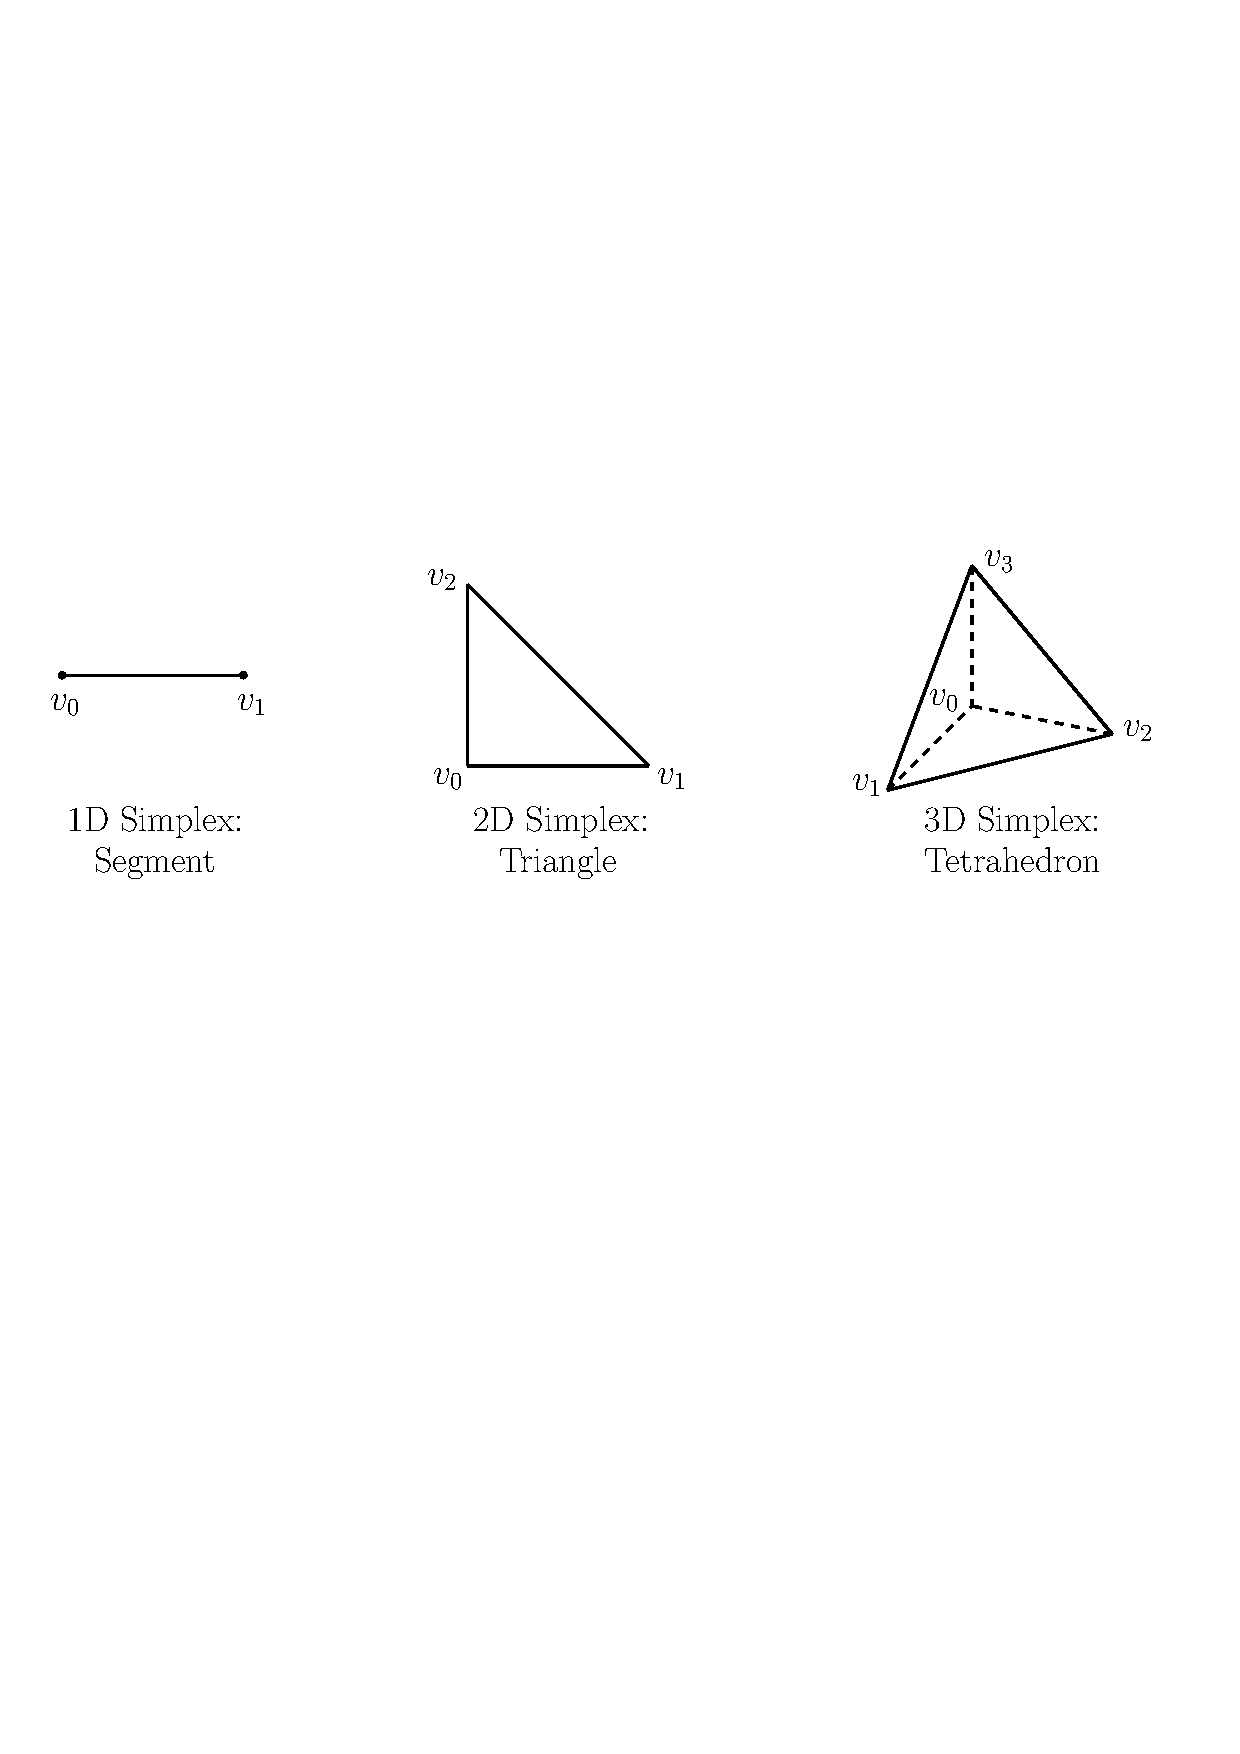
\includegraphics[scale=0.58]{./figures/AffineSimplices.pdf}
\caption{Simplices in 1D, 2D and 3D.}
\label{fig:affinesimplices}
\end{center}
\end{figure}

We now define the affine coordinates.
Let $ v_0,\ldots, v_N$, denote the vertices of some simplex, $\Delta$.
%\footnote{Segment ($N=1$), triangle ($N=2$), tetrahedron ($N=3$), etc.}
Any point $ x\in\Delta$ can be expressed as a convex combination of the vertices:
\begin{equation}
 x = \sum_{a=0}^N s_a v_a\, .\label{eq:affinerepresentation}
\end{equation}
The weights in the sum above, $s_0,\ldots,s_N$, are the affine coordinates for $\Delta$.
We can think of them both as coordinates in and of themselves, or functions of the Cartesian variable $x$. 
Due to being a convex combination, for all $x\in\Delta$ it holds that
\begin{equation}
\sum_{a=0}^N s_a(x)=1\,,\quad\text{ and }\quad s_a(x)\geq0\,.\label{eq:affinesumtoone}
\end{equation}

Throughout this document, to ease the understanding, we shall use the following convention for affine coordinates.
\begin{itemize}
	\item 1D: $\mu_0,\mu_1$ will be affine coordinates for edges ($N=1$, $\mu_a=s_a$ and $a=0,1$).
	\item 2D: $\nu_0,\nu_1,\nu_2$ will be affine coordinates for triangles ($N=2$, $\nu_a=s_a$ and $a=0,1,2$).
	\item 3D: $\lambda_0,\lambda_1,\lambda_2,\lambda_3$ will be affine coordinates for tetrahedra ($N=3$, $\lambda_a=s_a$ and $a=0,1,2,3$).
\end{itemize}
% $\mu_n:=s_n$, $n\in\{0,1\}$  (1D); $\nu_n:=s_n$, $n\in\{0,1,2\}$  (2D); $\lambda_n:=s_n$, $n\in\{0,1,2,3\}$ will denote affine coordinates for the tetrahedron (3D).
We will often use the following ``vector'' notation for compactness:
\begin{equation}
	\vec{s}_{ab}=(s_a,s_b)\,,\quad\qquad\vec{s}_{abc}=(s_a,s_b,s_c)\,,
\end{equation}
where $s=\mu,\nu,\lambda$. Hence, for example, $\vec{\nu}_{12}=(\nu_1,\nu_2)$ and $\vec{\lambda}_{031}=(\lambda_0,\lambda_3,\lambda_1)$.

Explicit formulas  for the affine coordinates (in terms of Cartesian coordinates) used for each element will be given at the beginning of each corresponding section.

% Throughout the text we will use the symbols
% $s_0,s_1,\ldots,s_N$ for $N=1,2,3$ to denote general affine coordinates. When the dimension of the space, $N$, is specified, then whenever possible, we will use the dimension-specific notations
% $\mu_0,\mu_1,\quad \text{in 1D},$
% $\nu_0,\nu_1,\nu_2\quad \text{in 2D},$
% $\lambda_0,\lambda_1,\lambda_2,\lambda_3\quad \text{in 2D},$
%  (define affine coordinates+notation)

\subsection{Outline}

The document will be organized naturally starting with the simplest element in 1D and then, as dimension and complexity increase, leading into the most complicated elements in 3D.
The order of sections is: segment (\S\ref{sec:Segment}), quadrilateral (\S\ref{sec:Quad}), triangle (\S\ref{sec:Tri}), hexahedron (\S\ref{sec:Hexa}), tetrahedron (\S\ref{sec:Tet}), prism (\S\ref{sec:Prism}) and pyramid (\S\ref{sec:Pyramid}).
Those interested only in simplicial elements may simply read segment, triangle and tetrahedron, while those interested only in quadrilateral and hexadedral elements can also skip the nonrelevant sections.
The prism and pyramid sections are better appreciated after reading through all of the previous sections.
As mentioned before, with regard to orientations, for each element there will always be a final subsection describing the necessary notions and modifications to implement orientation embedded shape functions.
Therefore, as a first iteration in trying to implement the shape functions, or for those readers for which this aspect is not of interest, we suggest skipping those subsections.
%These can be skipped by any reader for which this aspect is not of interest.

As a prelude to all the constructions, there is a section introducing the concept of polynomial scaling and the versions of Legendre and Jacobi polynomials used in our constructions.
More importantly, the concept of \textit{homogenization} is defined.
This is fundamental for the elements involving triangle faces (triangle, tetrahedron, prism, and pyramid).

Finally, as mentioned before, a set of tables available in Appendix \ref{app:ShapeFunctionTable} give a thorough definiton of all ancillary functions and shape functions presented in the text.
These tables should be used as a reference by the reader when looking at the provided code or when implementing their own version.
%Finally, should a reader wish immediately to skip the discussions, in Appendix~\ref{app:ShapeFunctionTable}, we provide a table giving a thorough definiton of all shape functions. This table should also be used as a reference when using or trying to implement the code.

\subsection{Previous Work}

Our constructions are often based either in part or in full in previous work by various collaborators in the field.
%The unique aspect here is the unified approach to all four 3D elements for the full sequence.
Construction of shape functions for the quadrilateral follows \citet{AinsworthCoyle01} (see also \citet{hpbook2}).

For the triangle and tetrahedron, our construction is based on the concept of \textit{scaled polynomials} as described by \citet{karniadakisbook}, \citet{Schoeberl_Zaglmayr_05}, \citet{SabineThesis} and the subsequent work of \citet{Beuchler_Pillwein_Schoeberl_Zaglmayr_12}.
%we initially follow the construction of \citet{Schoeberl_Zaglmayr_05} based on the idea of \textit{scaled polynomials}, and the subsequent work of \citet*{Beuchler_Pillwein_Schoeberl_Zaglmayr_12}.
See also \citet{Beuchler_Schoeberl_06, Beuchler_Pillwein_07, Beuchler_Pillwein_Zaglmayr_12} and \citet{Beuchler_Pillwein_Zaglmayr_13} for more details on obtaining good sparsity properties via appropriate selection of Jacobi polynomials.
Contrary to their work, here we study the classical $H(\text{curl})$ and $H(\text{div})$ conforming N\'{e}d\'{e}lec and Raviart-Thomas spaces having the property that they are affine invariant, and being compatible (at the space level) with the spaces proposed for the pyramid.
Other interesting shape functions for the tetrahedron include those of \citet{AinsworthBezier} based on Bernstein polynomials. Lastly, it is worth noting that \citet{SabineThesis} also presents a unified construction of the hexahedron and prism to complement the tetrahedron, but does not include the pyramid.

The prism element is a Cartesian product of the 2D triangle and 1D segment.
The prism shape functions therefore utilize constructs from the triangle and segment.

Construction of pyramid shape functions builds on the fundamental work of \citet{Nigam_Phillips_11} and their first family of pyramid spaces.
The spaces are natural for (parallelogram-based) affine pyramids, but as evidenced by \citet{Bergot_Durufle_14}, they also have other attractive properties in a non-affine setting.
We also note that \citet{Bergot_Gary_Durufle_10} and \citet{Bergot_Durufle_14} have contributed to the work on higher order pyramid shape functions, but their spaces and shape functions are different.
%Due to the pyramid being a connecting element, with very few elements in a typical mesh, our aim here is not to focus on the most optimal spaces for this element, but rather on the theoretical aspects of the commuting exact sequence property which ensure certain interpolation estimates.

The idea of orientation embedded shape functions follows the work of \citet{GattoDemkowicz10} and stems from discussions with Joachim Sch\"oberl dating back to the Vienna WCCM congress in 2002.

%and are compatible with the other classical N\'{e}d\'{e}lec's spaces of the first type.  , but based on this previous work, note the good properties this first family of spaces have in non-affine pyramids.
%We also stress that our aim in this work is not
%, we focus on the classical choice of spaces that contain only \Nedelec's tetrahedral polynomial spaces.
%{\color{red} whose elements?} These elements anticipate use of algebraic mesh generators and may fail to deliver optimal rates or may fail to even converge for general unstructured meshes (see \cite{hpbook2}, p.96, for a detailed discussion).


%\subsection{Outline}
%
%This paper is divided into isolated sections, one for each element the reader may wish to construct. Naturally, each section may require shape functions defined in the previous sections. For instance, to construct shape functions of the tetrahedron element, the reader must first be able to construct its trace spaces and so the segment and triangle element sections are somehow crucial. Naturally, the shape functions one needs for the tetrahedron are defined across the three sections on the segment (\S~\ref{sec:Segment}), the triangle (\S~\ref{sec:Tri}), and, of course, the tetrahedron (\S~\ref{sec:Tet}). However, we urge the reader to note that many sections are, in fact, independent of each other. For instance, if only reading for the tetrahedron, the reader may wish to skip both \S~\ref{sec:Quad} on the quadrilateral and \S~\ref{sec:Hexa} on the hexahedron even though they appear first. The shape functions in those two sections are not necessarily required for the tetrahedron as the geometry is different in each case beyond the level of the edge element.
%
%We advise all readers to read both \S~\ref{sec:Notation} and \S~\ref{sec:Segment}. The material in these sections is common to all elements, although the paricular discussion of Jacobi polynomials in \S~\ref{sec:Notation} is only required for elements having triangular faces.
%
%The shape functions of the pyramid element discussed in \S~\ref{sec:Pyramid} will require sections both \S~\ref{sec:Quad} on the quadrilateral and \S~\ref{sec:Tri} on the triangle. We also encourage the reader to browse \S~\ref{sec:Hexa} on the hexahedron and \S~\ref{sec:Tet} on the tetrahedron before seeking a full understanding of the pyramid element. Our construction for the pyramid is partially motivated by these previous sections.
%
%Should a reader wish immediately to skip to the discussion in any particular element, in Appendix~\ref{app:ShapeFunctionTable}, we provide a table giving a thorough definiton of all shape functions. This table should also be used as a reference when using the code.

